%!TEX root = ../../memoria.tex
\chapter{Avances}

% Sección que habla sobre los architecture en el framwork
%!TEX root = ../../../memoria.tex
\section{Arquitectura}\label{cap:arquitectura:section:generic_arquitectura}

\packagesAS es una estrategia de programación para \codeSeparationQA, \modularityAS, y \reusabilityQA. Al estructurar el código de cada \featureCPT en un \packagesAS separado, el código de una \featureCPT no tendrá acceso al código de otra \featureCPT excepto utilizando \exportCPT, haciendo cada dependencia explícita. Además esto permite la manera mas sencilla para realizar \testingCPT independientes a cada \featureCPT. Incluso es posible \publishINT los \packagesAS y utilizarlos en otros proyectos.

Es esta forma de estructurar el código la parte principal del desarrollo del \frameworkPC \ecommerceCOM. Cada vez que se requiera desarrollar una nueva solución específica utilizando el \frameworkPC, simplemente se incluirán todos aquellos \modulesAS necesarios para el desarrollo de la aplicación, y con un poco de desarrollo, obtener las \featuresCPT específicas buscadas.

Como este \frameworkPC será completamente \openSourcePC, la comunidad podrá crear nuevos \modulesAS con el fin de crear aquellas \featuresCPT que serán requeridos en el futuro.


% Nueva entrega
%  Meteor takes several existing tools and libraries; combines them with new
% thoughts and new libraries, standards, and services; and bundles them to provide
% an entire ecosystem for developing web and mobile applications that are a delight
% to use. 

% FEW CONVENTIONS ON STRUCTURE
% There are only few suggestions for structuring applications and code in Meteor. This
% freedom is great for single developers who can quickly hack on code, but it requires
% good coordination between team members when applications grow in size. It’s up to
% developers’ preference whether they use a single file or hundreds of folders and files.
% Some may embrace this freedom; others will find it necessary to define clear structures
% before being able to start coding.
Como se ha mencionado, \meteorNAME utiliza \librariesPC y \toolsCPT; las combina con nuevas consideraciones y nuevas \librariesPC, servicios y \standards; y las agrupa para proveer un ecosistema completo de desarrollo de aplicaciones \webINT y \mobileINT que da gusto utilizar. Sin embargo una de las devilidades que tiene 	\meteorNAME esta relacionado con las pocas convenciones para la estructura de aplicaciones y el código. Esta libertad o flexibilidad es aceptable para desarrolladores únicos quienes pueden rápidamente escribir código, pero esto requiere una muy buena coordinacion entre miembros de un equipo cuando la aplicación crece en tamaño. Todo depende de la preferencia de los desarrolladores si utilizar un solo archivo o cientos de carpetas y archivos. Para resolver este problema se propondra una estructura, apoyada por una variedad de \packagesAS para el desarrollo de grandes aplicaciones en las que usualmente serán desarrolladas por equipos de trabajo.

\subsection{\packagesAS desarrollados por la comunidad}
Una gran cantidad de soluciones han sido desarrolladas por la comunidad para solucionar problemas altamente comunes a la hora de desarrollar aplicaciones. A continuación dichos \packagesAS serán nombrados y descritos.

	\begin{itemize}
		\item
			\textbf{\nameCollectionTwo}. Permite asociar un \schemaDB a un \mongoCollection. Autáticamente se valida la la estructura cuando se inserta o actualiza desde el \clientAS o el \serverAS. Esto es altamente deseable principalmente por que asegura que solo propiedas y valores aceptables puedan ser insertados desde el \clientAS. De esta manera, inserciones y actualizaciones \clientSideAS pueden ser permitidas sin comprometer seguridad o integridad de la información.
		\item
			\textbf{\nameRouter}. Un enrutador que funciona en el \serverAS y en el \browserINT, diseñado especificamente para \meteorNAME.
		\item
			\textbf{\nameCollectionHooks}. Extiende \mongoCollection con \hooksCPT \beforeAfterDB para \insertDB, \updateDB, \removeDB, \findDB y \findOneDB.
		\item
			\textbf{\nameBower}. \bowerIONAME es un repositorio popular de librerias \javaScriptNAME \clientSideAS.
		\item
			\textbf{\securityPackage}. Es un \packageAS de \meteorNAME que proporciona un lenguage \apiAS simple y lógico para definir seguridad para las \collectionsMETEOR de \mongodbNAME. Agrega funcionalidades al \coreAS de  seguridad \allowdenyCPT.
			% A Meteor package that provides a simple, logical, plain language API for defining write security on your MongoDB collections. Wraps the core allow/deny security.
		\item
			\textbf{\velocityCorePackage}. El \testRunnerCPT \reactive para \meteorNAME.
			% The reactive test-runner for Meteor.
		\item
			\textbf{\sanjoJasminePackage}. Corresponde a la integración de \meteorNAME \velocityNAME para el \frameworkPC de \testingCPT \jasmineNAME 2.3. Facilita el proceso de \testingCPT en la aplicación y los \packageAS de \meteorNAME con \testsCPT unitarios e integrados.
			% The Meteor Velocity integration for the Jasmine 2.3 testing framework. Makes it easy to test your Meteor app and packages with unit and integration tests.
		\item
			\textbf{\bunyanPackage}. Exporta y agrega el \moduleAS de \loggingCPT \bunyanNAME. También agrega el \clientAS \browserifyNAME y \bunyanprettyStreamMETEOR.
			% Add and export the Bunyan logging module, also add the browserify client and bunyan-prettystream.
		\item
			\textbf{\dThreePackage}. \dddNAME es una \libraryPC	\javaScriptNAME para la manipulación de  \documentsDB basados en datos. \dThreePackage facilita el proceso de publicación de datos utilizando \htmlNAME, \svgNAME Y \cssNAME. \dThreePackage enfatiza el uso de \webStandardINT permite el uso de todas las opciones disponibles en los \browsersINT modernos, sin la necesidad de utilizar un \frameworkPC propietario, combinando componentes visuales y un acercamiento a \dataDrivenCPT para la manipulación de \htmldomNAME.
			% D3.js is a JavaScript library for manipulating documents based on data. D3 helps you bring data to life using HTML, SVG and CSS. D3’s emphasis on web standards gives you the full capabilities of modern browsers without tying yourself to a proprietary framework, combining powerful visualization components and a data-driven approach to DOM manipulation.
		\item
			\textbf{\undStringLatestPackage}. \undStringLatestMETEOR \packageAS para \meteorNAME. Es una librería para la manipulación de \stringsPL.
			%underscore.string repackaged for Meteor
			% The underscore.string string manipulation library repackaged for Meteor.
		\item
			\textbf{\lessPackage}. \lessNAME extiende \cssNAME con comportamientos dinámicos tales como variables, \mixinsNAME, operaciones y funciones. Esto permite  \stylesheetsNAME mas compactos y ayuda a la reducción de duplicación en los archivos \cssNAME. 

			%LESS extends CSS with dynamic behavior such as variables, mixins, operations and functions. It allows for more compact stylesheets and helps reduce code duplication in CSS files.

			%With the less package installed, .less files in your application are automatically compiled to CSS and the results are included in the client CSS bundle.

			%If you want to @import a file, give it the extension .import.less to prevent Meteor from processing it independently.
		\item
			\textbf{\bootstrapPackage}. Este \packageAS integra \bootstrapNAME en \meteorNAME permitiendo configurar lo que realmente se necesita.
			%This package integrates bootstrap into meteor and lets you configure what parts you need.
	\end{itemize}


\section{Estructura propuesta para el desarrollo de grandes aplicaciones}\label{cap:arquitectura:section:generic_architecture_structure}

Cuando se comienza a trabajar en \meteorNAME es importante entender que código es ejecutado en que ambiente al momento de escribir aplicaciones. En teoría, todo el código puede correr en cualquier parte en el \stackAS, pero existen algunas limitaciones. \apikeyAS no deberian enviarse al \clientAS; los \events que manejan los \clicks del \mouse no son útiles en el \serverAS. Para indicar a \meteorNAME donde ejecutar código específico, es posible organizar código en carpetas dedicadas o utilizar un \checkCPT para verificar en que contexto estan corriendo.

En \meteorNAME existen directorios especiales que separan logicamente el alcance de su contenido. Estos directorios se pueden apreciar en la \refFigura{esquema:simple_structure_meteor}.


	\begin{itemize}
		\item
			\textbf{\clientFolder}. Todo el código que se encuentre dentro de la carpeta  \clientFolder solo será visible desde el \clientSideAS.
		\item
			\textbf{\serverFolder}.  Todo el contenido de la carpeta \serverFolder estará disponible solo para el \serverSideAS.
		\item
			\textbf{\publicFolder}. Los archivos dentro de esta carpeta son visibles desde el \clientSideAS y \serverSideAS.
		\item
			\textbf{\privateFolder}. Los archivos dentro de esta carperta se pueden acceder solo desde el código del \serverAS a traves de un \apiAS de \assetsAS.
			%These files can only be accessed by server code through Assets API and are not accessible to the client.
	\end{itemize}

% Estructura bàsica de Meteor
%!TEX root = ../../memoria.tex
\begin{figure}[h!]
	\centering
		\tikzstyle{every node}=[draw=black,thick,anchor=west,inner sep=2pt,minimum size=1pt]
		\tikzstyle{selected}=[draw=cyan,fill=cyan!30]
		\begin{tikzpicture}[
			grow via three points={one child at (0.5,-0.7) and
			two children at (0.5,-0.7) and (0.5,-1.4)},   
			edge from parent path={(\tikzparentnode.south) |- (\tikzchildnode.west)}]
			\node {carpeta proyecto/}
			child {	node [label={[xshift=6.0cm, yshift=-0.58cm, color=gray] Estructura Básica}]{client/}
			    child {	node [draw=none] {main.html}}
			    child { node [draw=none] {...}}
			    child { node {resources/}
		        	child { node [draw=none] {onload.js}}
		        	child { node [draw=none] {main.css}}
		        	child { node [draw=none] {...}}
			    }
		    	child [missing] {}
			}
			child [missing] {}
			child [missing] {}
			child [missing] {}
			child [missing] {}
			child [missing] {}
			child {node {public/}
				child { node [draw=none] {validations.js}}
				child { node [draw=none] {...}}
			}
			child [missing] {}
			child [missing] {}
			child { node {server/}
			    child { node [draw=none] {business logic.js}}
			    child { node [draw=none] {...} }
		    }
		    child [missing] {}
			child [missing] {}
			child { node {private/}
			    child { node [draw=none] {...}}
		    };
		\end{tikzpicture}
		\tikzstyle{every node}=[] % resets borders of tables
		\tikzstyle{selected}=[] % resets selected
	\caption{Estructra simple de una aplicación en \meteorNAME.}
	\label{esquema:simple_structure_meteor}
\end{figure}

El código compartido es especialmente útil para el desarrollo de aplicaciones. A modo de ejemplo, en el caso de las validaciones, el mismo método es utilizado tanto en el \clientSideAS como en el \serverSideAS. En el \clientSideAS utilizado para mostrar un mensaje de error en el \browserINT (un rut mal escrito), y en el \serverSideAS para no persistir información incorrecta en la \dataBaseDB.

Para definir una estructura de desarrollo, se debe considerar, entre otras cosas,  que paradigma de programación se esta utilizando, cuales son sus principios, y el \apiAS que este proporciona. Se procede entonces a definir ciertos conceptos relevantes:

	\begin{itemize}
		\item
			% In Meteor, views are defined in templates. A template is a snippet of HTML that can include dynamic data. You can also interact with your templates from JavaScript code to insert data and listen to events.
			\textbf{\templatesMETEOR}. En \meteorNAME, las \viewsAS son definidas en \templatesMETEOR. Un \templateMETEOR es una pequeña porcion de \htmlNAME que puede incluir datos dinámicos. Incluso es posible interactuar con el \templateMETEOR desde código \javaScriptNAME para insertar información y escuchar \events \cite{online_meteor_documentation}.
		\item
			\textbf{\sessionMETEOR}. Provee un objeto global en el \clientAS que puede utilizarse para guardar un arbitrario par \keyValueDB. \cite{online_meteor_documentation}.
		\item
			\textbf{\trackerMETEOR}. \meteorNAME tiene sistema simple de dependencia para hacer \trackingMETEOR, permitiendo así automáticamente \rerunCPT \templatesMETEOR y otras funciones siempre que variables \sessionMETEOR, consultas a la \dataBaseDB, y otros recursos de datos cambien \cite{online_meteor_documentation}.
		\item
			\textbf{\collectionsMETEOR}. \meteorNAME guarda la información en \collectionsMETEOR. Objetos \javaScriptNAME almacenados en \collectionsMETEOR son denominados \documentsDB \cite{online_meteor_documentation}.

		\item
			\textbf{\publishsubscribeMETEOR}. El \serverAS de \meteorNAME puede publicar un conjunto de \documentsDB , y los \clientsAS pueden subscribirse a esas publicaciones. \cite{online_meteor_documentation}.
	\end{itemize}

Teniendo estas consideraciones en mente, se define la siguiente estructura global para el desarrollo de una aplicación cualquiera.

% Estructura global de una aplicación en Meteor
%!TEX root = ../../memoria.tex
\begin{figure}[h!]
	\centering
	\scaleCommandTreeFolder
		\tikzstyle{every node}=[draw=black,thick,anchor=west,inner sep=2pt,minimum size=1pt]
		\tikzstyle{selected}=[draw=cyan,fill=cyan!30]
		\begin{tikzpicture}[scale=(\scaleValueTreeFolder),
			grow via three points={one child at (0.5,-0.7) and
			two children at (0.5,-0.7) and (0.5,-1.4)},   
			edge from parent path={(\tikzparentnode.south) |- (\tikzchildnode.west)}]
			\node {carpeta proyecto}
				child { node {client/}}
				child { node {bin/}}
				child { node {server/}}
				child { node {private/}}
				child { node {public/}}
				child { node {common/}}
				child { node {lib/}}
				child { node {docs/}}
				child { node {settings/}}
				child { node {packages/}}
				child { node [draw=none] {package.js} }
				child { node [draw=none] {README.md} }
				child { node [draw=none] {LICENSE.md} }
		    ;
		\end{tikzpicture}
		\tikzstyle{every node}=[] % resets borders of tables
		\tikzstyle{selected}=[] % resets selected
	\caption{Estructra global para una aplicación en \meteorNAME.}
	\label{esquema:gloal_structure_meteor_app}
\end{figure}

% Estructura de la carpeta bin de una aplicación en Meteor
%!TEX root = ../../memoria.tex
\begin{figure}[h!]
	\centering
	\scaleCommandTreeFolder
		\tikzstyle{every node}=[draw=black,thick,anchor=west,inner sep=2pt,minimum size=1pt]
		\tikzstyle{selected}=[draw=cyan,fill=cyan!30]
		\begin{tikzpicture}[scale=(\scaleValueTreeFolder),
			grow via three points={one child at (0.5,-0.7) and
			two children at (0.5,-0.7) and (0.5,-1.4)},   
			edge from parent path={(\tikzparentnode.south) |- (\tikzchildnode.west)}]
			\node {bin/}
				child { node {helpers/}}
				child { node {templates/}}
				child { node [draw=none] {...}}
				child { node [draw=none] {collection-dump}}
				child { node [draw=none] {debug}}
				child { node [draw=none] {deploy}}
				child { node [draw=none] {dump}}
				child { node [draw=none] {install}}
				child { node [draw=none] {reset}}
				child { node [draw=none] {run}}
				child { node [draw=none] {test}}
				child { node [draw=none] {...}};
		\end{tikzpicture}
		\tikzstyle{every node}=[] % resets borders of tables
		\tikzstyle{selected}=[] % resets selected
	\caption{Estructra de la carpeta \folderBin para una aplicación en \meteorNAME.}
	\label{esquema:bin_structure_meteor_app}
\end{figure}

Como se mecionó, \clientFolder es la carpeta que es solo visible desde el \clientSideAS, lo que significa que contiene solo código útil para el \clientAS. Su estructura básica se puede observar en \refFigura{esquema:client_structure_meteor_app}; y cada una de sus partes corresponden a:

	\begin{itemize}
		\item
			\textbf{\helpersMETEOR/}. Carpeta donde se encuentran todos los \helpersMETEOR globales del sistema.
		\item
			\textbf{\templatesMETEOR/} Contiene los \templatesMETEOR y sus respectivos \helpersMETEOR. Se utiliza el mismo nombre en ambos archivos, con el fin de identificarlos. En \refFigura{esquema:template_structure_meteor_app} se muestra con detalle esta carpeta.
		\item
			\textbf{app.coffee}. Lugar donde estan todas aquellas funciones y variables globales del sistema.
		\item
			\textbf{subscriptions.coffee}. Lugar donde se especifican todas subscripciones a las diferentes publicaciones que proporciona el \serverAS.
	\end{itemize}

% Estructura de la carpeta client de una aplicación en Meteor
%!TEX root = ../../memoria.tex
\begin{figure}[h!]
	\centering
	\scaleCommandTreeFolder		
		\tikzstyle{every node}=[draw=black,thick,anchor=west,inner sep=2pt,minimum size=1pt]
		\tikzstyle{selected}=[draw=cyan,fill=cyan!30]
		\begin{tikzpicture}[ scale=(\scaleValueTreeFolder),
			grow via three points={one child at (0.5,-0.7) and
			two children at (0.5,-0.7) and (0.5,-1.4)},   
			edge from parent path={(\tikzparentnode.south) |- (\tikzchildnode.west)}]
			\node {client/}
				child { node {helpers/}}
				child { node {templates/}}
				child { node [draw=none] {...}}
				child { node [draw=none] {app.coffee}}
				child { node [draw=none] {subscriptions.coffee}}
				child { node [draw=none] {...}};
		\end{tikzpicture}
		\tikzstyle{every node}=[] % resets borders of tables
		\tikzstyle{selected}=[] % resets selected
	\caption{Estructra de la carpeta \clientFolder para una aplicación en \meteorNAME.}
	\label{esquema:client_structure_meteor_app}
\end{figure}

La carpeta 	\templateMETEOR tiene el suficiente detalle y relevancia como para indicar sus partes.

\begin{itemize}
	\item
		\textbf{\folderAccount/}. Contiene los \templatesMETEOR y \helpersMETEOR necesarios para manegar las cuentas de usuarios. 
	\item
		\textbf{\folderDashboard/}. Aca estan todos los archivos necesrios(\templatesMETEOR y \helpersMETEOR) para el manejo de la interfaz de administrador. Dada su naturaleza, es esperable que se agreguen una gran cantidad de carpetas dentro.
	\item
		\textbf{\folderLayout/}. Contiene todos aquellos \templatesMETEOR con sus respectivos \helpersMETEOR que son globales en el sistema. Como por ejemplo las alertas, el encabezado, el pie de página, \loadingCPT, e interfaces estáticas tales como: acceso no autorizado, página no encontrada, recurso no encontrado, etc. Es importante agregar que estas interfaces estáticas, no cuentan con \helpersMETEOR; la razón tras esto es que el encargado de manejar esos \templatesMETEOR es el \packagesAS \nameRouter.
	\item
		\textbf{Carpetas exclusivas del proyecto}. Aca deberian ir las carpetas que separen lógicamente las diferentes funcionalidades de la aplicación que se desea realizar. A modo de ejemplo, en el proyecto que se esta realizando en este memoria, se han creado carpetas para el carro de compras y los productos respectivamente.
\end{itemize}

% Estructura de la carpeta client de una aplicación en Meteor
%!TEX root = ../../memoria.tex
\begin{figure}[h!]
	\centering
	\scaleCommandTreeFolder		
		\tikzstyle{every node}=[draw=black,thick,anchor=west,inner sep=2pt,minimum size=1pt]
		\tikzstyle{selected}=[draw=cyan,fill=cyan!30]
		\begin{tikzpicture}[ scale=(\scaleValueTreeFolder),
			grow via three points={one child at (0.5,-0.7) and
			two children at (0.5,-0.7) and (0.5,-1.4)},   
			edge from parent path={(\tikzparentnode.south) |- (\tikzchildnode.west)}]
			\node {template/}
				child { node {accounts/}
					child { node [draw=none] {accounts.coffee}}
					child { node [draw=none] {accounts.html}}
					child { node [draw=none] {...}}
				}
				child [missing] {}
				child [missing] {}
				child [missing] {}
				child { node {dashboard/}
					child { node {accounts/}
						child { node [draw=none] {accounts.coffee}}
						child { node [draw=none] {accounts.html}}
					}
					child [missing] {}
					child [missing] {}
					child { node [draw=none] {...}}
				}
				child [missing] {}
				child [missing] {}
				child [missing] {}
				child [missing] {}
				child { node {layout/}
					child { node {alerts/}}
					child { node {footer/}}
					child { node {header/}
						child { node [draw=none] {header.coffee}}
						child { node [draw=none] {header.html}}
						child { node [draw=none] {...}}
					}
					child [missing] {}
					child [missing] {}
					child [missing] {}
					child { node {loading/}
						child { node [draw=none] {loading.html}}
					}
					child [missing] {}
					child { node {notFound/}
						child { node [draw=none] {notFound.html}}
					}
					child [missing] {}
					child { node {notice/}
						child { node [draw=none] {unauthorized.html}}
						child { node [draw=none] {...}}
					}
					child [missing] {}
					child [missing] {}
					child { node [draw=none] {layout.coffee}}
					child { node [draw=none] {layout.html}}
				}
				child [missing] {}
				child [missing] {}
				child [missing] {}
				child [missing] {}
				child [missing] {}
				child [missing] {}
				child [missing] {}
				child [missing] {}
				child [missing] {}
				child [missing] {}
				child [missing] {}
				child [missing] {}
				child [missing] {}
				child [missing] {}
				child [missing] {}
				child { node [draw=none] {...}};
		\end{tikzpicture}
		\tikzstyle{every node}=[] % resets borders of tables
		\tikzstyle{selected}=[] % resets selected
	\caption{Estructra de la carpeta \folderTemplate para una aplicación en \meteorNAME.}
	\label{esquema:template_structure_meteor_app}
\end{figure}

\begin{itemize}
	\item
		\textbf{\folderCollections/}. Aca se crean las variables de todas las \collectionsMETEOR definidas en la aplicación. Aunque es totalmente posible crear variables propias para el \clientAS como para el \serverAS; se considera una buena práctica hacerlo de esta manera.
	\item
	 	\textbf{\folderHooks/}. Contiene los \hooksCPT relacionados con los \collectionsMETEOR. Código escrito en base al \packagesAS \nameCollectionHooks.
	\item
		\textbf{\folderSchemas/}. Contiene todos los \schemasDB que se han creado utilizando el \packagesAS \collectionsMETEOR.
	\item
		\textbf{packageGlobals.js}. Contiene todas las variables globales del sistema. En este caso, tambien son variables que se encuentran en el \environmentPL del \clientAS y del \serverAS.
	\item
		\textbf{routing.coffee}. Contiene todo el código relacionado con el enrutamiento. El código es desarrollado utilizando el \packagesAS \nameRouter.
\end{itemize}

% Estructura de la carpeta common de una aplicación en Meteor
%!TEX root = ../../memoria.tex
\begin{figure}[h!]
	\centering
	\scaleCommandTreeFolder
		\tikzstyle{every node}=[draw=black,thick,anchor=west,inner sep=2pt,minimum size=1pt]
		\tikzstyle{selected}=[draw=cyan,fill=cyan!30]
		\begin{tikzpicture}[scale=(\scaleValueTreeFolder),
			grow via three points={one child at (0.5,-0.7) and
			two children at (0.5,-0.7) and (0.5,-1.4)},   
			edge from parent path={(\tikzparentnode.south) |- (\tikzchildnode.west)}]
			\node {common/}
				child { node {collections/}}
				child { node {hooks/}}
				child { node {schemas/}}
				child { node [draw=none] {common.coffee}}
				child { node [draw=none] {helpers.coffee}}
				child { node [draw=none] {routing.coffee}}
				child { node [draw=none] {packageGlobals.coffee}}
				child { node [draw=none] {...}}
		    ;
		\end{tikzpicture}
		\tikzstyle{every node}=[] % resets borders of table
		\tikzstyle{selected}=[] % resets selected
	\caption{Estructra de la carpeta \folderCommon para una aplicación en \meteorNAME.}
	\label{esquema:common_structure_meteor_app}
\end{figure}

La carpeta \folderDocs (\refFigura{esquema:docs_structure_meteor_app}) contiene toda la documentación de la aplicación, lo que incluye información sobre \deploymentCPT, \packagesAS, \routingAS, \templatesMETEOR, agradecimientos, convenciones, etc.

% Estructura de la carpeta docs de una aplicación en Meteor
%!TEX root = ../../memoria.tex
\begin{figure}[h!]
	\centering
	\scaleCommandTreeFolder
		\tikzstyle{every node}=[draw=black,thick,anchor=west,inner sep=2pt,minimum size=1pt]
		\tikzstyle{selected}=[draw=cyan,fill=cyan!30]
		\begin{tikzpicture}[scale=(\scaleValueTreeFolder),
			grow via three points={one child at (0.5,-0.7) and
			two children at (0.5,-0.7) and (0.5,-1.4)},   
			edge from parent path={(\tikzparentnode.south) |- (\tikzchildnode.west)}]
			\node {docs/}
				child { node [draw=none] {conventions.md}}
				child { node [draw=none] {deploying.md}}
				child { node [draw=none] {fixtures.md}}
				child { node [draw=none] {installation.md}}
				child { node [draw=none] {methods.md}}
				child { node [draw=none] {...}}
		    ;
		\end{tikzpicture}
		\tikzstyle{every node}=[] % resets borders of tables
		\tikzstyle{selected}=[] % resets selected
	\caption{Estructra de la carpeta \folderDocs para una aplicación en \meteorNAME.}
	\label{esquema:docs_structure_meteor_app}
\end{figure}

La carpeta \folderLib contiene todas las librerias. Como se observa en \refFigura{esquema:lib_structure_meteor_app}, existe una carpeta y un archivo \jsonNAME llamados \folderBower. A traves del \packagesAS \nameBower se manejan las diferentes librerias necesarias.
% Estructura de la carpeta lib de una aplicación en Meteor
%!TEX root = ../../memoria.tex
\begin{figure}[h!]
	\centering
	\scaleCommandTreeFolder
		\tikzstyle{every node}=[draw=black,thick,anchor=west,inner sep=2pt,minimum size=1pt]
		\tikzstyle{selected}=[draw=cyan,fill=cyan!30]
		\begin{tikzpicture}[scale=(\scaleValueTreeFolder),
			grow via three points={one child at (0.5,-0.7) and
			two children at (0.5,-0.7) and (0.5,-1.4)},   
			edge from parent path={(\tikzparentnode.south) |- (\tikzchildnode.west)}]
			\node {lib/}
				child { node {bower/}}
				child { node [draw=none] {bower.json}}
				child { node {css/}}
		    ;
		\end{tikzpicture}
		\tikzstyle{every node}=[] % resets borders of tables
		\tikzstyle{selected}=[] % resets selected
	\caption{Estructra de la carpeta \folderLib para una aplicación en \meteorNAME.}
	\label{esquema:lib_structure_meteor_app}
\end{figure}


La carpeta \privateFolder se utiliza principalmente para mantener archivos \jsonNAME que contienen \collectionsMETEOR con la información suficiente para realizar la \localisationPC, además de guardar los archivos necesarios para \fixturesPC.

% Estructura de la carpeta private de una aplicación en Meteor
%!TEX root = ../../memoria.tex
\begin{figure}[h!]
	\centering
		\tikzstyle{every node}=[draw=black,thick,anchor=west,inner sep=2pt,minimum size=1pt]
		\tikzstyle{selected}=[draw=cyan,fill=cyan!30]
		\begin{tikzpicture}[
			grow via three points={one child at (0.5,-0.7) and
			two children at (0.5,-0.7) and (0.5,-1.4)},   
			edge from parent path={(\tikzparentnode.south) |- (\tikzchildnode.west)}]
			\node {private/}
				child { node {data/}}
				child { node [draw=none] {...}}
				child { node [draw=none] {readme.md}}
				child { node [draw=none] {...}}
		    ;
		\end{tikzpicture}
		\tikzstyle{every node}=[] % resets borders of tables
		\tikzstyle{selected}=[] % resets selected
	\caption{Estructra de la carpeta \privateFolder para una aplicación en \meteorNAME.}
	\label{esquema:private_structure_meteor_app}
\end{figure}

La carpeta \folderTests (representada en la \refFigura{esquema:tests_structure_meteor_app}) contiene los archivos para realizar \testingCPT a la aplicación. Las pruebas se realizan apoyados en el \packageAS \sanjoJasminePackage.

% Estructura de la carpeta tests de una aplicación en Meteor
%!TEX root = ../../memoria.tex
\begin{figure}[h!]
	\centering
		\tikzstyle{every node}=[draw=black,thick,anchor=west,inner sep=2pt,minimum size=1pt]
		\tikzstyle{selected}=[draw=cyan,fill=cyan!30]
		\begin{tikzpicture}[
			grow via three points={one child at (0.5,-0.7) and
			two children at (0.5,-0.7) and (0.5,-1.4)},   
			edge from parent path={(\tikzparentnode.south) |- (\tikzchildnode.west)}]
			\node {test/}
				child { node {resources/}
		        	child { node {jasmine}
		        		child { node {client/}
		        			child { node [draw=none] {...}}
		        		}
		        		child [missing] {}
		        		child { node {server/}
		        			child { node [draw=none] {...}}
		        		}
		        	}
			    }
		    ;
		\end{tikzpicture}
		\tikzstyle{every node}=[] % resets borders of tables
		\tikzstyle{selected}=[] % resets selected
	\caption{Estructra de la carpeta \folderTests para una aplicación en \meteorNAME.}
	\label{esquema:tests_structure_meteor_app}
\end{figure}

La carpeta \serverFolder, como su nombre lo indica, contiene la implementación de la aplicación solo visible por el \serverSideAS. De los archivos existentes, podemos destacar:

\begin{itemize}
	\item
		\textbf{publications.coffee}. Archivo que contiene todas las publicaciones de \documentsDB. Cada una de estas publicaciones pueden incluir definiciones de seguridad relacionadas con roles para limitar la entrega.
	\item
	 	\textbf{security.coffee}. Archivo que contiene todas las reglas de seguridad para \insertsDB, \updatesDB y \removesDB iniciadas desde código inesguro (\clientsAS). De todas maneras, existen otras acciones para ciertos roles que tienen permitido realizar. Dichas acciones no necesariamente aparecen aquí si la operación de \dataBaseDB es ejecutada desde un método del \serverAS. Las definiciones de seguridad aqui descritas utilizan el \packageAS \securityPackage.
 	\item
	 	\textbf{fixture.coffee}. Su principal función es ejecutar el código de inicio de \fixturesPC. Este código es ejecutado solo la primera vez, para poblar la \dataBaseDB con las \collectionsMETEOR requeridas como mínimo, para realizar \testingCPT y/o poder ejecutar la aplicación. Algo muy relevante que se crea, es el usuario \textbf{Administrador}.  Esta ejecución se inicia con el evento de inicio de \meteorNAME.
	\item
	 	\textbf{app.coffee}. Contiene información relacionada con los niveles de \bunyanNAME (\packageAS \bunyanPackage) que se utilizan para hacer \loggingCPT; junto con algunas funciones principales del servidor.
\end{itemize}

% Estructura de la carpeta server de una aplicación en Meteor
%!TEX root = ../../memoria.tex
\begin{figure}[h!]
	\centering
		\tikzstyle{every node}=[draw=black,thick,anchor=west,inner sep=2pt,minimum size=1pt]
		\tikzstyle{selected}=[draw=cyan,fill=cyan!30]
		\begin{tikzpicture}[
			grow via three points={one child at (0.5,-0.7) and
			two children at (0.5,-0.7) and (0.5,-1.4)},   
			edge from parent path={(\tikzparentnode.south) |- (\tikzchildnode.west)}]
			\node {server/}
				child { node {buildtools/}}
				child { node {methods/}}
				child { node [draw=none] {...}}
				child { node [draw=none] {app.coffee}}
				child { node [draw=none] {factories.coffee}}
				child { node [draw=none] {publications.coffee}}
				child { node [draw=none] {fixtures.coffee}}
				child { node [draw=none] {register.coffee}}
		    ;
		\end{tikzpicture}
		\tikzstyle{every node}=[] % resets borders of tables
		\tikzstyle{selected}=[] % resets selected
	\caption{Estructra de la carpeta \serverFolder para una aplicación en \meteorNAME.}
	\label{esquema:server_structure_meteor_app}
\end{figure}


\section{Requisitos  que \folderAccount}


% Sección que habla sobre los architecture en el framwork
%!TEX root = ../../../memoria.tex
\section{Arquitectura del \frameworkPC}\label{cap:arquitectura:section:arquitectura_framework}

\subsection{\packagesAS}

A continuación se describe las funcionalidades de cada uno de los \packagesAS que actualmente existen. La estructura se encuentra en \refFigura{cap:avances:current_architecture}.

\tikzset{
  basic/.style  = {draw, text width=2cm, drop shadow, font=\sffamily, rectangle},
  root/.style   = {basic, rounded corners=2pt, thin, align=center,
                   fill=green!30},
  level 2/.style = {basic, rounded corners=6pt, thin,align=center, fill=green!60,
                   text width=8em},
  level 3/.style = {basic, thin, align=left, fill=pink!60, text width=6.5em}
}
\begin{figure}[H]
	\centering
	
	
	\begin{tikzpicture}[
	  level 1/.style={sibling distance=40mm},
	  edge from parent/.style={->,draw},
	  >=latex]

	% root of the the initial tree, level 1
	\node[root] {\rtcom}
	% The first level, as children of the initial tree
	  child {node[level 2] (c1) {\rtcomCorePCKG}}
	  child {node[level 2] (c2) {\helloworldPCKG}}
	  child {node[level 2] (c3) {\rtcomSearchPCKG}}
	  %child {node[level 2] (c4) {rtcom-shipping}}
	 % child {node[level 2] (c5) {rtcom-paypal}}
	  child {node[level 2] (c6) {\rtcomGoogleanalPCKG}};

	\end{tikzpicture}
	\caption{\architectureCPT actual de la solución.}
	\label{cap:avances:current_architecture}
\end{figure}
	\begin{itemize}
		\item
			\textbf{\rtcom} es un \frameworkPC \ecommerceCOM desarrollado con \meteorNAME, \nodejsNAME, \mongodbNAME, \coffeescript con un enfoque \reactive y \realTimeINT.
		\item
			\textbf{\rtcomCorePCKG} corresponde al \coreAS de la solución. Contiene todas aquellas \featuresCPT básicas y \templatesAS a una plataforma \ecommerceCOM tales como manejo de \itemsCOM, \sessionsINT, etc. De momento he trabajado solo con esas dos \featuresCPT.
		\item
			\textbf{\rtcomGoogleanalPCKG} es el \moduleAS para \googleanalytics. Aunque no se encuentra completamente integrado, si genera datos.
		\item
			\textbf{\helloworldPCKG} es un \moduleAS para prueba de conceptos.
	\end{itemize}


La arquitectura descrita en la \refSection{cap:arquitectura:section:generic_arquitectura} fue diseñada para facilitar las implementaciones de cada uno de los \packagesAS que se desarrollen en los proyectos de \meteorNAME. En particular para el proyecto que se desarrolla en este informe se utiliza dicha estructura principalmente en el \packagesAS \coreAS de la aplicación.

\subsubsection{\rtcomCorePCKG}

Como su nombre lo indica, este \packagesAS corresponde al \coreAS del \frameworkPC conteniendo todas aquellas caracteristicas intrínsecas que dan vida a un sitio \ecommerceCOM. 

\subsubsection{\rtcomCoreThemePCKG}

Este \packagesAS es la base del \bootstrap \themeCPT del \frameworkPC de \ecommerceCOM. Este contiene todos los archivos \lessNAME utilizados para el proceso que genera los archivos \lessNAME personalizado para el \frameworkPC. Este \packagesAS puede ser copiado para crear \themeCPT adicinales para el \frameworkPC \ecommerceCOM.

La implementación de este \packagesAS esta soportada sobre \bootstrapPackage permitiendo sencillamente hacer todas aquellas configuraciones que se desean. \bootstrapPackage permite, entre otras cosas, indicar exactamente cuales son las componentes de \bootstrapNAME que se desean utilizar, así como personalizar e importar el \themeCPT.

A modo de ejemplo, se mostrarán a continuación ejemplos de importaciones de \themesCPT en el \frameworkPC. Para esto se utilizará los \themesCPT gratuitos que proporciona \bootswatchNAME. Esta tarea es muy sencilla, y basta con agregar el \refsource{source:less:generic_bootswatch_theme} al final del arhivo generado por \bootstrapPackage llamado \textbf{custom.reaction.import.less}.

% import codigo 
%%!TEX root = ../../../memoria.tex

\medskip
\begin{lstlisting}[caption= Código genérico para importar \themesCPT de ., label=source:less:generic_bootswatch_theme]
	@import "http://bootswatch.com/THEME_NAME/bootswatch.less";
	@import "http://bootswatch.com/THEME_NAME/variables.less";
\end{lstlisting}
\medskip
\begin{lstlisting}[caption= Código genérico para importar \themesCPT desde \bootswatchNAME, label=source:less:generic_bootswatch_theme]
	@import "http://bootswatch.com/THEME-NAME/bootswatch.less";
	@import "http://bootswatch.com/THEME-NAME/variables.less";
\end{lstlisting}

En donde \textbf{THEME-NAME} corresponde a algún \themeCPT de los disponibles en el sitio de \bootswatchNAME. En particular, los \themesCPT \textbf{\themeSandstone}, \textbf{\themeJournal}, \textbf{\themeCyborg} y \textbf{\themeSuperHero} se pueden apreciar en la \refFigura{figure:bootstrap:theme_standstone}, \refFigura{figure:bootstrap:theme_journal}, \refFigura{figure:bootstrap:theme_cyborg} y \refFigura{figure:bootstrap:theme_superhero} respectivamente.


\begin{figure}[H]
	\centering
	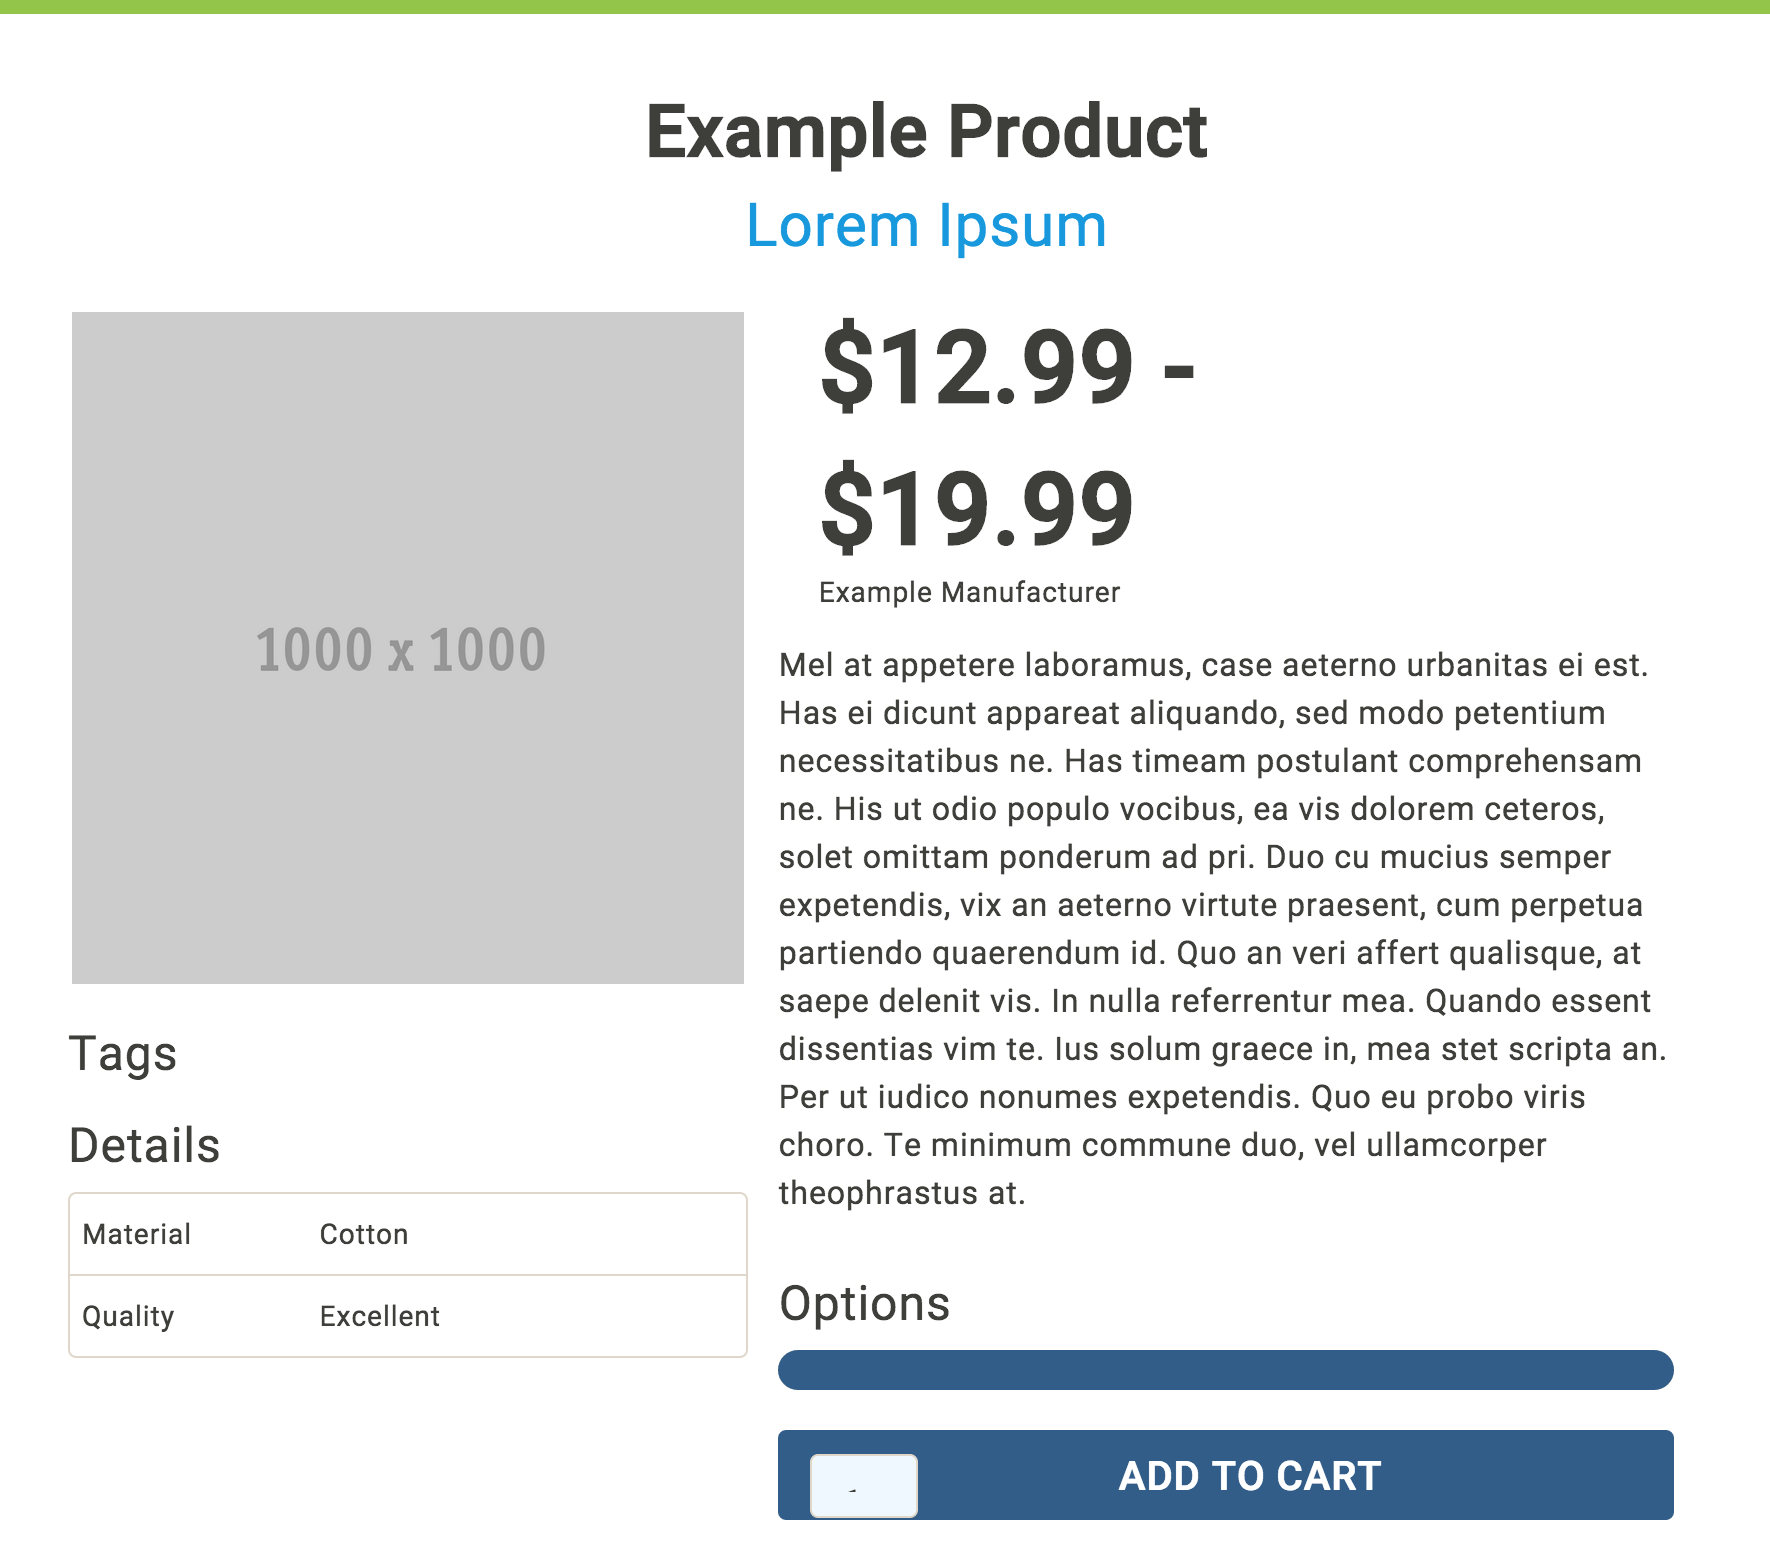
\includegraphics[width=0.6\textwidth]{figuras/bootstrap/bootstrap_theme_sandstone.png}

	\caption{Descripción de un producto utilizando el \themeCPT \textbf{\themeSandstone} del sitio \bootswatchNAME.}
	\label{figure:bootstrap:theme_standstone}
\end{figure}

\begin{figure}[H]
	\centering
	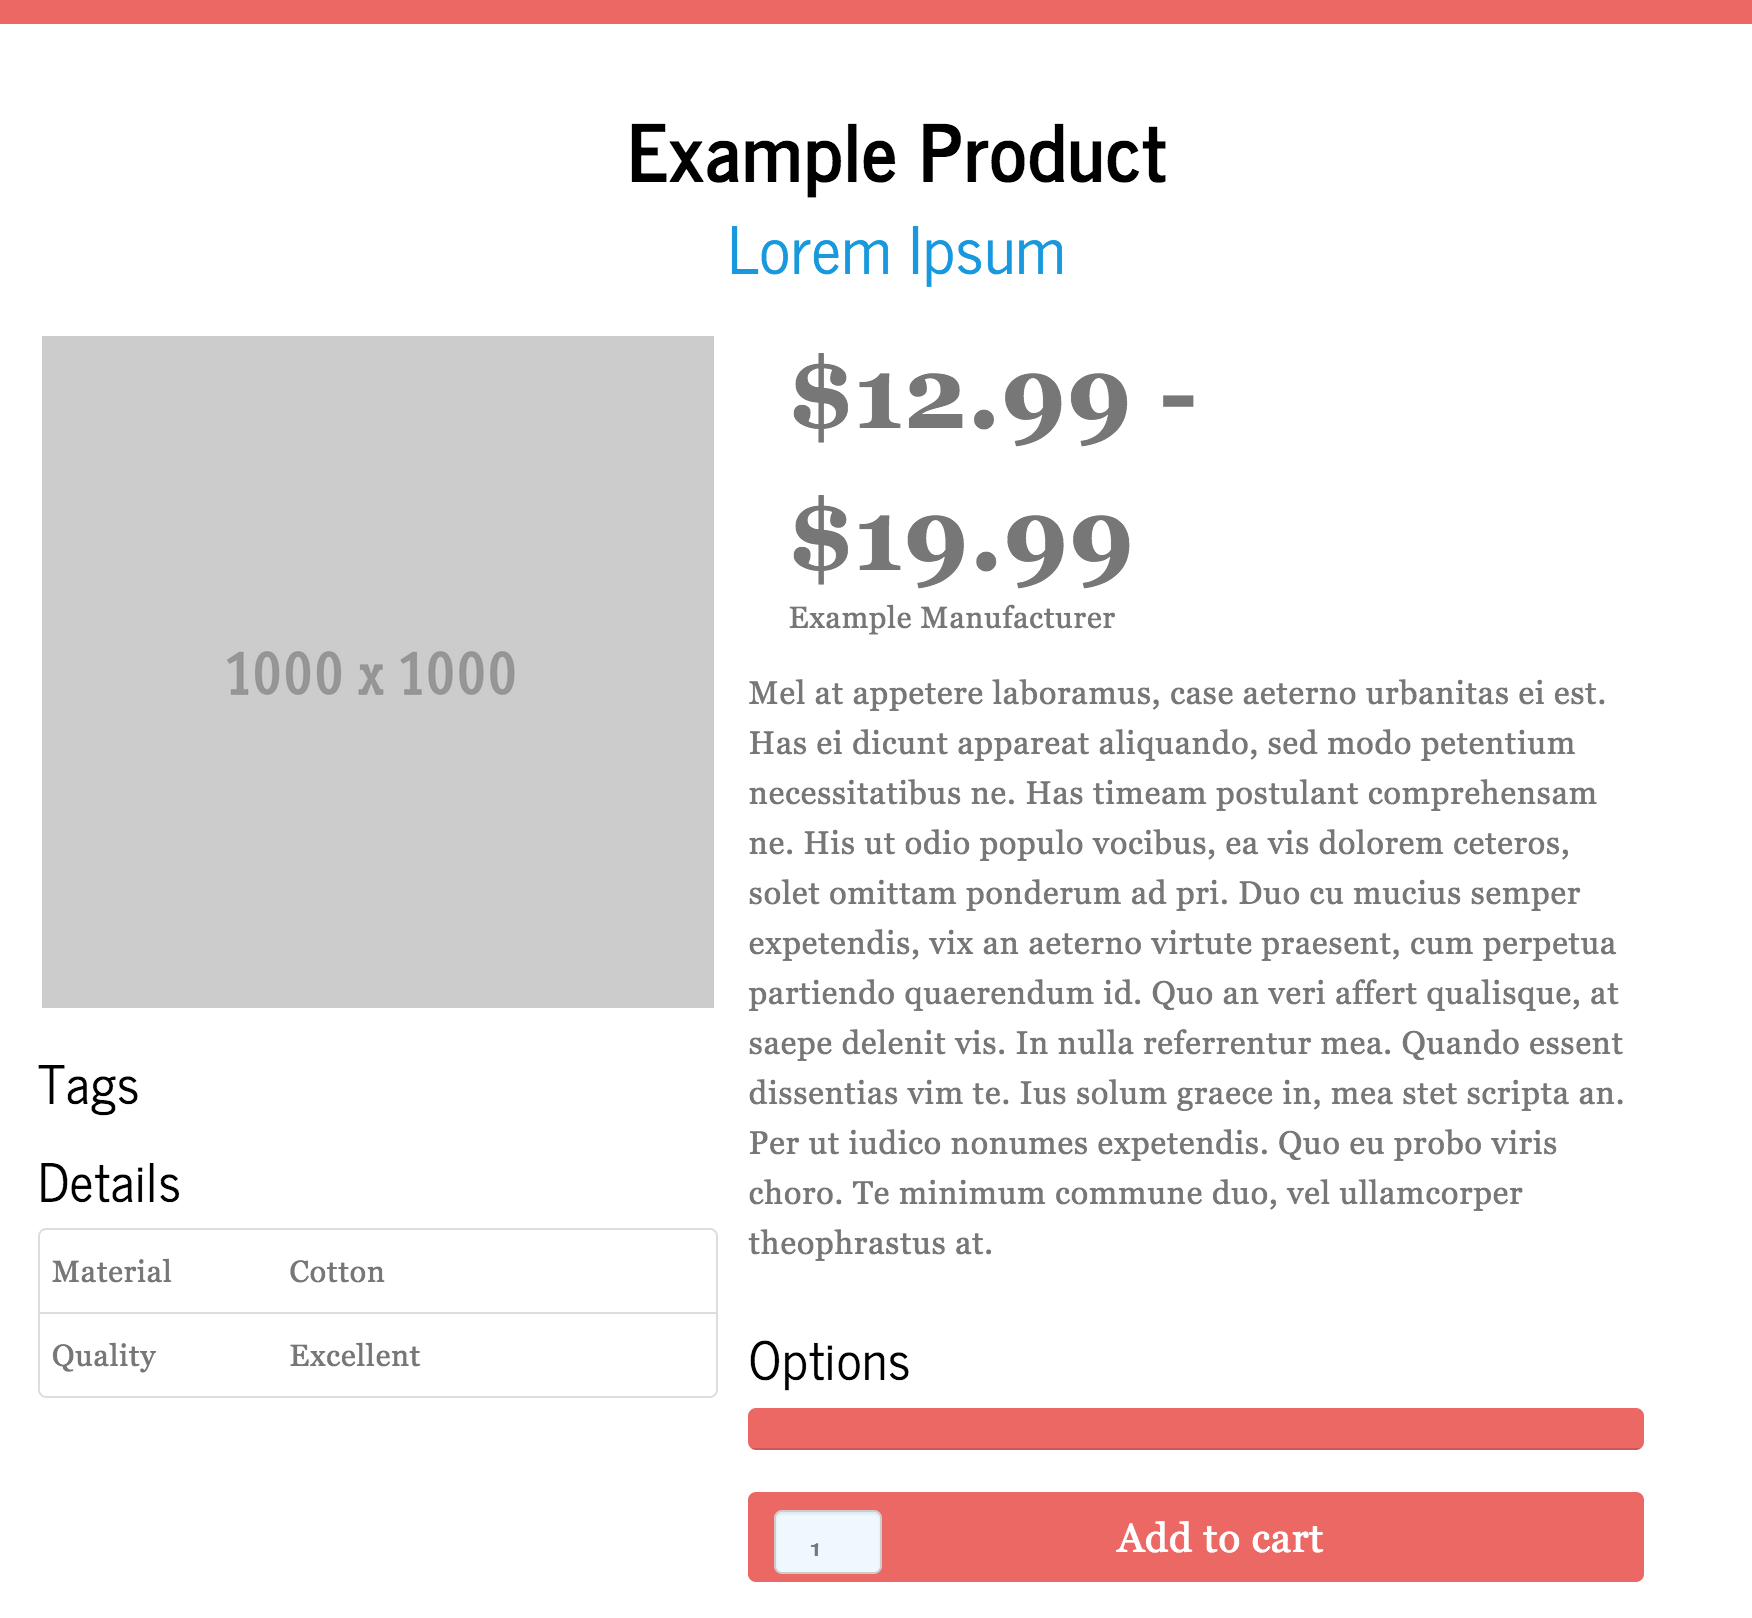
\includegraphics[width=0.6\textwidth]{figuras/bootstrap/bootstrap_theme_journal.png}

	\caption{Descripción de un producto utilizando el \themeCPT \textbf{\themeJournal} del sitio \bootswatchNAME.}
	\label{figure:bootstrap:theme_journal}
\end{figure}

\begin{figure}[H]
	\centering
	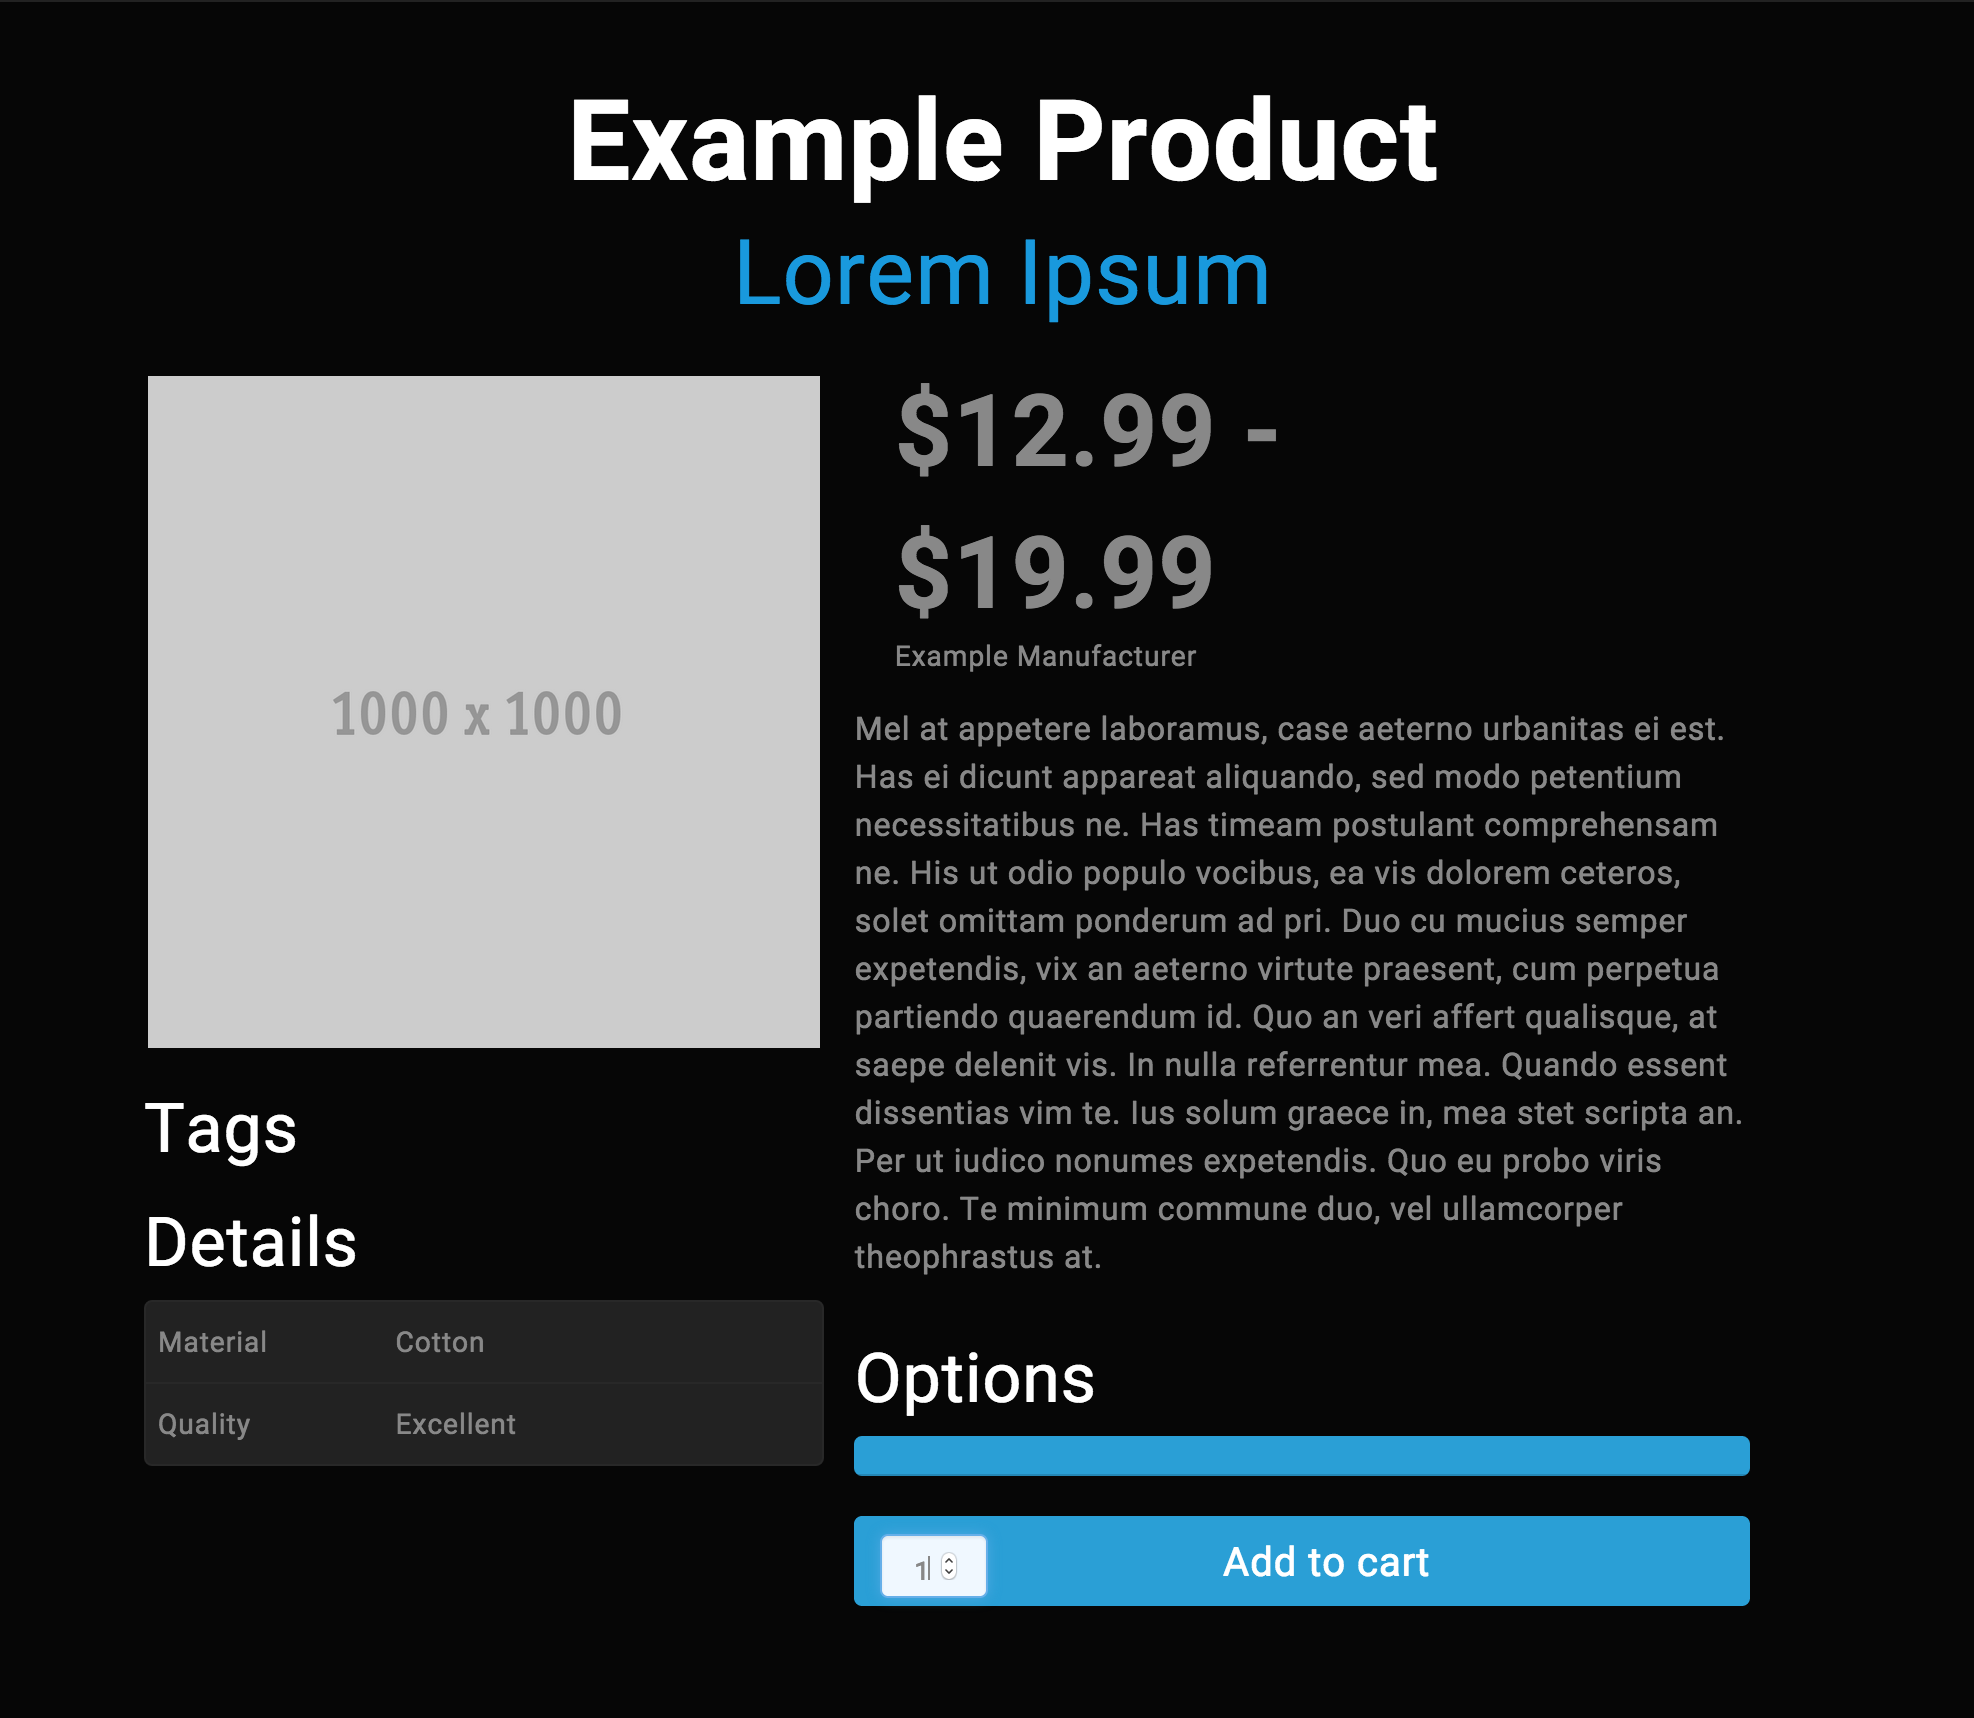
\includegraphics[width=0.6\textwidth]{figuras/bootstrap/bootstrap_theme_cyborg.png}

	\caption{Descripción de un producto utilizando el \themeCPT \textbf{\themeCyborg} del sitio \bootswatchNAME.}
	\label{figure:bootstrap:theme_cyborg}
\end{figure}


\begin{figure}[H]
	\centering
	\includegraphics[width=0.6\textwidth]{figuras/bootstrap/bootstrap_theme_superhero.png}

	\caption{Descripción de un producto utilizando el \themeCPT \textbf{\themeSuperHero} del sitio \bootswatchNAME.}
	\label{figure:bootstrap:theme_superhero}
\end{figure}


% Sección que habla sobre los workflows en el framwork
%!TEX root = ../../../memoria.tex

\subsection{\workflowsCPT}

%TODO
% Introduccion de workflows

Existen una serie de pasos que se pueden experimentar al visitar un sitio \ecommerceCOM, entre los cuales podemos destacar:

	\begin{itemize}
		\item
			\textbf{Shopping Experience}.
		\item
			\textbf{Order Capture} 
		\item
			\textbf{Order Fullfillment} 
		\item
			\textbf{Order processing}
		\item
			\textbf{Shipping} 
		\item
			\textbf{Customer Files} 
		\item
			\textbf{Paymanat Sistems} 
		\item
			\textbf{Customer Service} 
		\item
			\textbf{Accounting} 
		\item
			\textbf{Returning} 
	\end{itemize}


Cada uno de los pasos dentro de un \workflowsCPT puede ser considerado como un estado el cual cambiará dependiendo de los eventos que esten involucrados. Por lo tanto cada uno de estos \workflowsCPT puede ser modelado utilizando una máquina de estados finitos.
Para el caso particular del \frameworkPC para \ecommerceCOM, 4 han sido los \workflowsCPT que han sido implementados utilizando la librería \javaScriptNAME \finiteStateMachine.

\begin{figure}[H]
	\centering
	\includegraphics[width=1.1\textwidth]{figuras/cart_state_machine.jpg}

	\caption{Máquina de estado de carro de compras.}
	\label{figure:cart_state_machine}
\end{figure}


\begin{figure}[H]
	\centering
	\includegraphics[width=0.8\textwidth]{figuras/order_state_machine.jpg}

	\caption{Máquina de estado del estado de una orden.}
	\label{figure:order_state_machine}
\end{figure}



% caracteristicas actuales en funcionamiento
%!TEX root = ../../../memoria.tex
\section{Características actuales}

Como se explico en la \refSection{cap:arquitectura:section:generic_architecture_structure}, fue necesario desarrollar una arquitectura genérica para el desarrollo de aplicaciones en \meteorNAME con el fin de generar código de calidad. Acto seguido se comenzo con la implementación de las siguientes características:

\subsection{Cuestas de usuarios}
 
%Meteor Accounts
%Meteor Accounts is a complete user account system that you can drop into your application. With one line of code, you can have login, logout, account creation, email validation, password recovery, and login with OAuth providers like Facebook or Twitter.
Existe un sistema completo de cuentas de usuarios el cual permite hacer \loginCPT(\refFigura{figure:account:sign_in_ui}), \logoutCPT(\refFigura{figure:account:log_out}), creación de cuentas (\refFigura{figure:account:create_account}), y recuperacion de contraseña(\refFigura{figure:account:reset_password}). Aunque en estricto rigor, la recuperación de contraseña momentaneamente corresponde a una contraseña aleatoria generada por la aplicación y enviada al correo.

\begin{figure}[H]
	\centering
	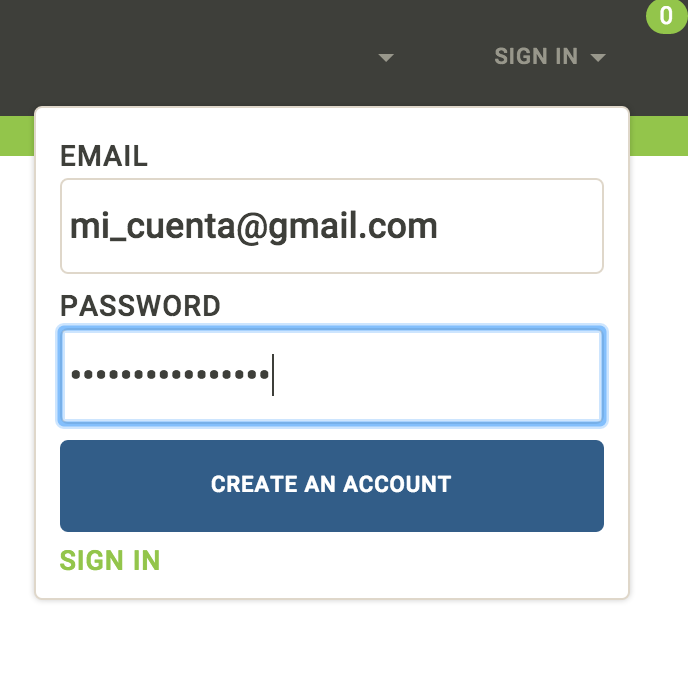
\includegraphics[width=0.3\textwidth]{figuras/accounts/create_account.png}

	\caption{Creación de una cuenta.}
	\label{figure:account:create_account}
\end{figure}

\begin{figure}[H]
	\centering
	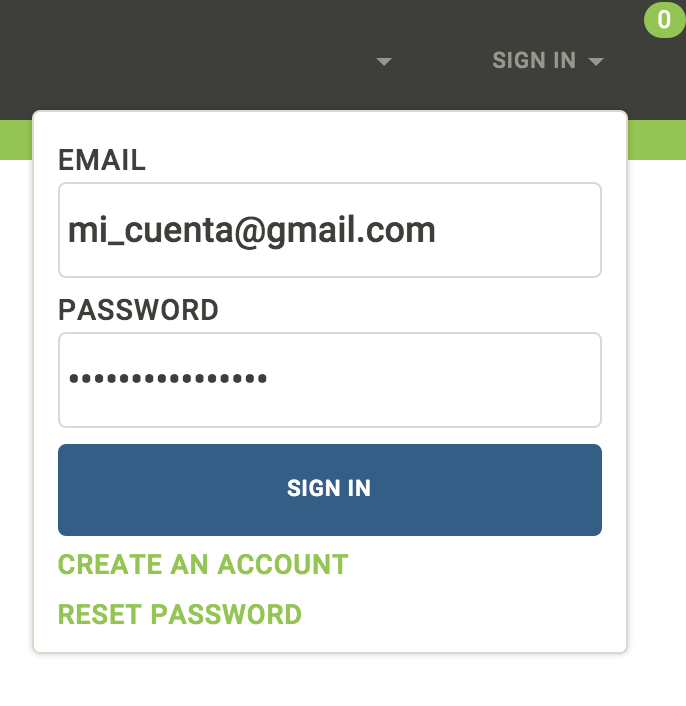
\includegraphics[width=0.3\textwidth]{figuras/accounts/sign_in_ui.png}

	\caption{Autenticarse en la aplicación.}
	\label{figure:account:sign_in_ui}
\end{figure}


\begin{figure}[H]
	\centering
	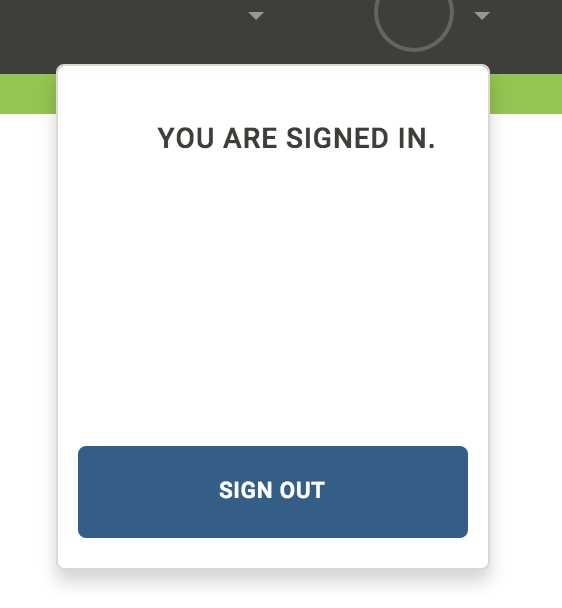
\includegraphics[width=0.3\textwidth]{figuras/accounts/log_out.png}

	\caption{Desvincular la cuenta de la aplicación.}
	\label{figure:account:log_out}
\end{figure}

\begin{figure}[H]
	\centering
	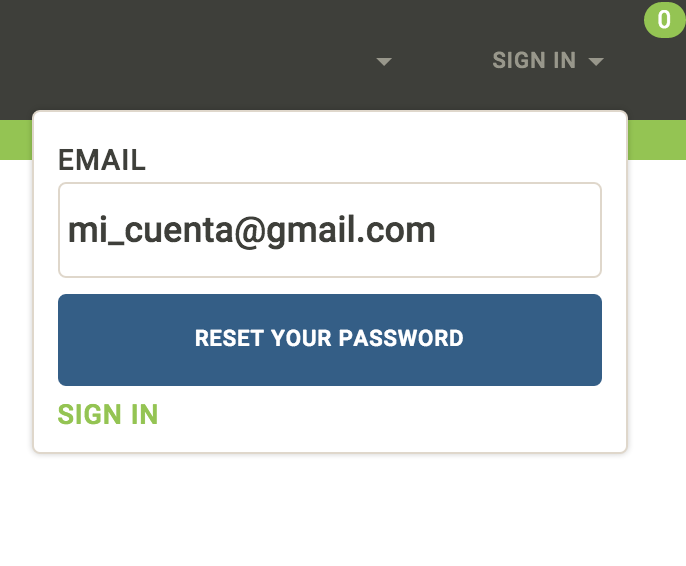
\includegraphics[width=0.3\textwidth]{figuras/accounts/reset_password.png}

	\caption{Reset contraseña.}
	\label{figure:account:reset_password}
\end{figure}

Además el sistema permite hacer \loginCPT a traves de un servicio de autenticación \thirdParty tales como \facebook, \googleNAME, \twitterNAME, \gitHubNAME, entre otros utilizando los \packagesAS de \meteorNAME \accountFacebook, \accountGoogle, \accountTwitter y \accountGithub respectivamente. En la \refFigura{figure:account:log_in_plus_facebook} se observa la existencia de un servicio \thirdParty para la autenticación en la aplicación.


\begin{figure}[H]
	\centering
	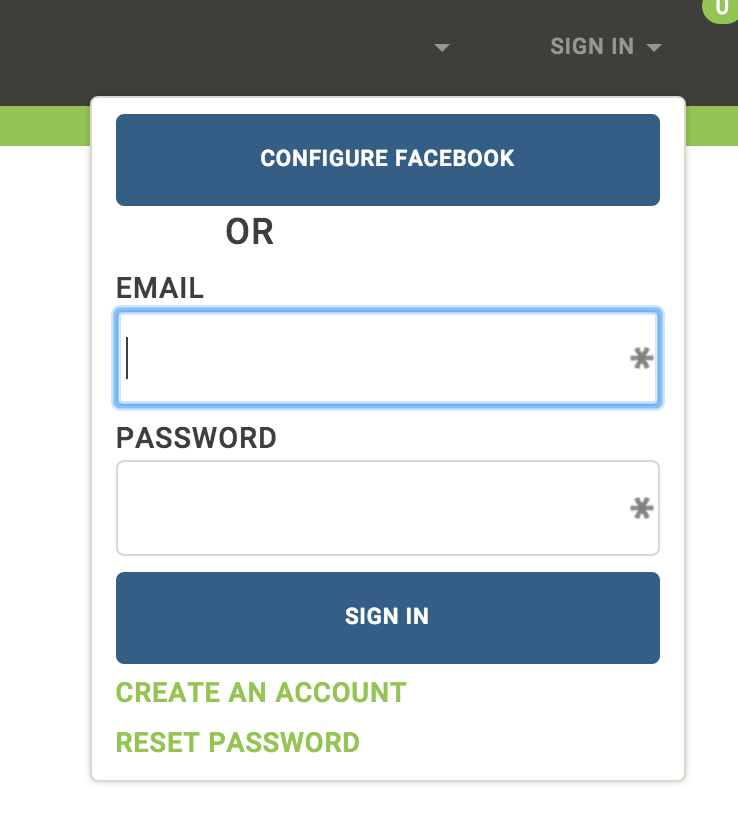
\includegraphics[width=0.3\textwidth]{figuras/accounts/log_in_plus_facebook.png}

	\caption{Autenticarse utilizando un servicio \thirdParty.}
	\label{figure:account:log_in_plus_facebook}
\end{figure}

Es importante agregar que el sistema automáticamente agrega en la interfaz la opción de autenticarse utilizando el servicio \thirdParty simplemente agregando el \packagesAS de \meteorNAME; y por consiguiente este desaparecerá si el \packagesAS es removido. En la \refFigura{figure:account:log_in_all_package} se aprecian varios servicios \thirdParty para la autenticación de la aplicación.

\begin{figure}[H]
	\centering
	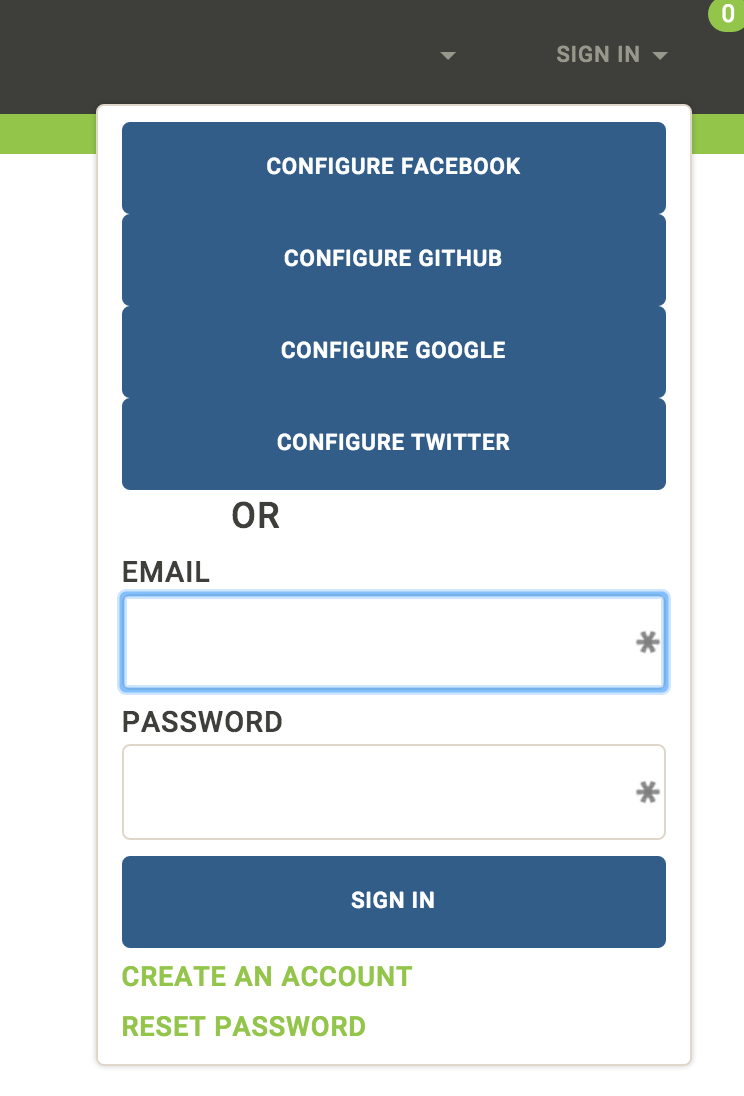
\includegraphics[width=0.3\textwidth]{figuras/accounts/log_in_all_package.png}

	\caption{Autenticarse utilizando uno de varios servios \thirdParty.}
	\label{figure:account:log_in_all_package}
\end{figure}


%you can provide your own UI for these features or you can even use a premade boilerplate UI to get up and running quickly.

%eteor Accounts is a modular system, and anyone can write a package that provides a new login method. Some, but not all of these packages are officially maintained by the Meteor Project. For example, accounts-password has a complete password-based login system, including password recovery. Packages such as accounts-google, accounts-facebook, and accounts-twitter provide the ability to log in with common third-party authentication services.

%The account database is stored in a users database collection that is automatically created on the server. Currently this can only be stored in MongoDB, but other databases will likely be supported in the future, depending on demand. The schema of this database is shown in the main Meteor docs.

%Passwords are safely encoded with bcrypt according to industry best practices.

% \subsection{Localización}

% Ingles no solo ostenta el primer lugar como el idioma más utilizado. \rankingCPT que considera además del porcentage de población, la distribución geográfica. Si no que además es el idioma más utilizado en los \websitesINT alcanzando la cifra de 59,4\%. Seguido tímidamente por Rusia con un 5.9\% \cite{online_world_wide_languages}. Mirando estas cifras se podría concluir que la inclusión de múltiples idiomas en un \siteINT \ecommerceCOM	no reprensentaría ingresos importantes.
% El potencial económico \online es de \$45 trillones, de acuerdo a un estudio realizado por \commonSenseAdvisoryNAME \cite{online_world_global_oportunity_multi_languages}.  Sin una solida estrategia de localización que considere \websitesINT \ecommerceCOM con multi-idiomas, será  un desafio tener al alcanze de la mano ese \revenueCOM. De hecho, el mismo estudio vislumbró que si solo se tiene una versión en ingles del  \siteINT, se estará limitado solo a una tercera parte del total.

% %Grow revenue with website localization
% %The economic potential of online communication is $45 trillion, according to a recent study by Common Sense Advisory. How exciting! The sky is the limit for your global business.
% %Or is it?
% %Without a solid localization strategy that incorporates an e-commerce website in multiple languages, it will be a challenge to get within arm’s reach of this revenue. In fact, the same study found that if you have just an English version of your website, you’re limited to only one third of the pot.

% ¿Cuántos serán los idiomas necesarios para permanecer competitivo en el mundo \online. Los investigadores dicen que un mínimo de 14. Las marcar mundiales que aspiran a un 95\% de las billeteras \online necesitan de 20 idiomas. Si bien es cierto, no es siempre posible mantener contenido \online en 20 idiomas, es dificil negar los beneficios de la localización para regiones específicas al rededor del mundo \cite{online_world_global_oportunity_multi_languages}. Estan son las razones de por que se considera muy importante la localización en el \frameworkPC y de por que se aborda esta caracteristica desde los inicios.

% Actualmente la aplicación cuenta con un sistema robusto para la localización, permitiendo nuevos idiomas simplemente agregando un archivo \jsonNAME. En la \refFigura{figure:features:languages_available}
%How many languages does it take for global businesses to stay competitive online? The research says a minimum of 14. Global brands wanting to appeal to 95 percent of the world’s online wallet need 20 languages. While it isn’t always feasible for a business to translate online content into 20 languages, it’s hard to deny the benefits of website localization for targeted regions around the world.
%Many businesses recognize this and plan to add even more languages to their localization strategy in the future. One example is European-based clothing seller ASOS. They launched a website for the Chinese and Russian markets in 2013 to expand their global footprint. They already had a presence in the United Kingdom, United States, France, Germany and Australia. They saw international sales overall increase by 39 percent with their past website localization initiatives—so they knew that additional language sites would help grow revenue.
%If you’re ready to get a bigger piece of the global e-commerce pie, like ASOS, consider upping the number of languages on your website. Check out the article, Global e-commerce: Are these 5 items in your localization shopping cart?, for tips on how to approach e-commerce website localization.


% \begin{figure}[H]
% 	\centering
% 	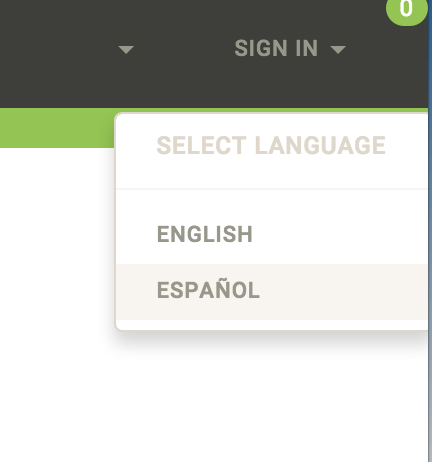
\includegraphics[width=0.3\textwidth]{figuras/languages_available.png}

% 	\caption{Selección de idioma para el \websitesINT.}
% 	\label{figure:features:languages_available}
% \end{figure}


% \subsection{Descripción de un producto}

% La aplicación permite consultar la descripción de un producto. Dicha interfaz puede observarse en la \refFigura{figure:bootstrap:theme_cyborg}. Se puede aprenciar alguans de las carecteristicas de las que ya dispone cada producto.

% \begin{itemize}
% 	\item
% 		Un título del producto.
% 	\item
% 		Un subtítulo para dar un resumen.
% 	\item
% 		Un espacio para la foto del producto.
% 	\item
% 		Un lugar para la descripción del producto.
% 	\item
% 		Un precio ó intervalo de precios.
% \end{itemize}

% Si bien es cierto, esta interfaz no tiene aún todas las caracteristicas usualmente visibles en los \websitesINT \ecommerceCOM típicos, son un paso intermedío hacia esa finalidad.

%  \subsection{Edición de un producto}

% Actualmente puede asociarce un creador a un producto (usando \fixturesPC) y por lo tanto solo aquel tendra acceso a editar, eliminar, y proximamente ocultar el producto.

% Para editar los campos, simplemente es necesario seleccionar la componente con el \mousePC y hacer un \click. La componente cambiara su aspecto para dar \feedback al usuario de que esta seleccionada la componente y que puede realizar ediciones sobre el campo. En la \refFigura{figure:features:interfaz_edicion_producto}, \ref{figure:features:interfaz_edicion_editando_description} y \ref{figure:features:interfaz_edicion_editando_subtitulo} es posible apreciar la componenete que se ha seleccionado para editar.

% \begin{figure}[H]
% 	\centering
% 	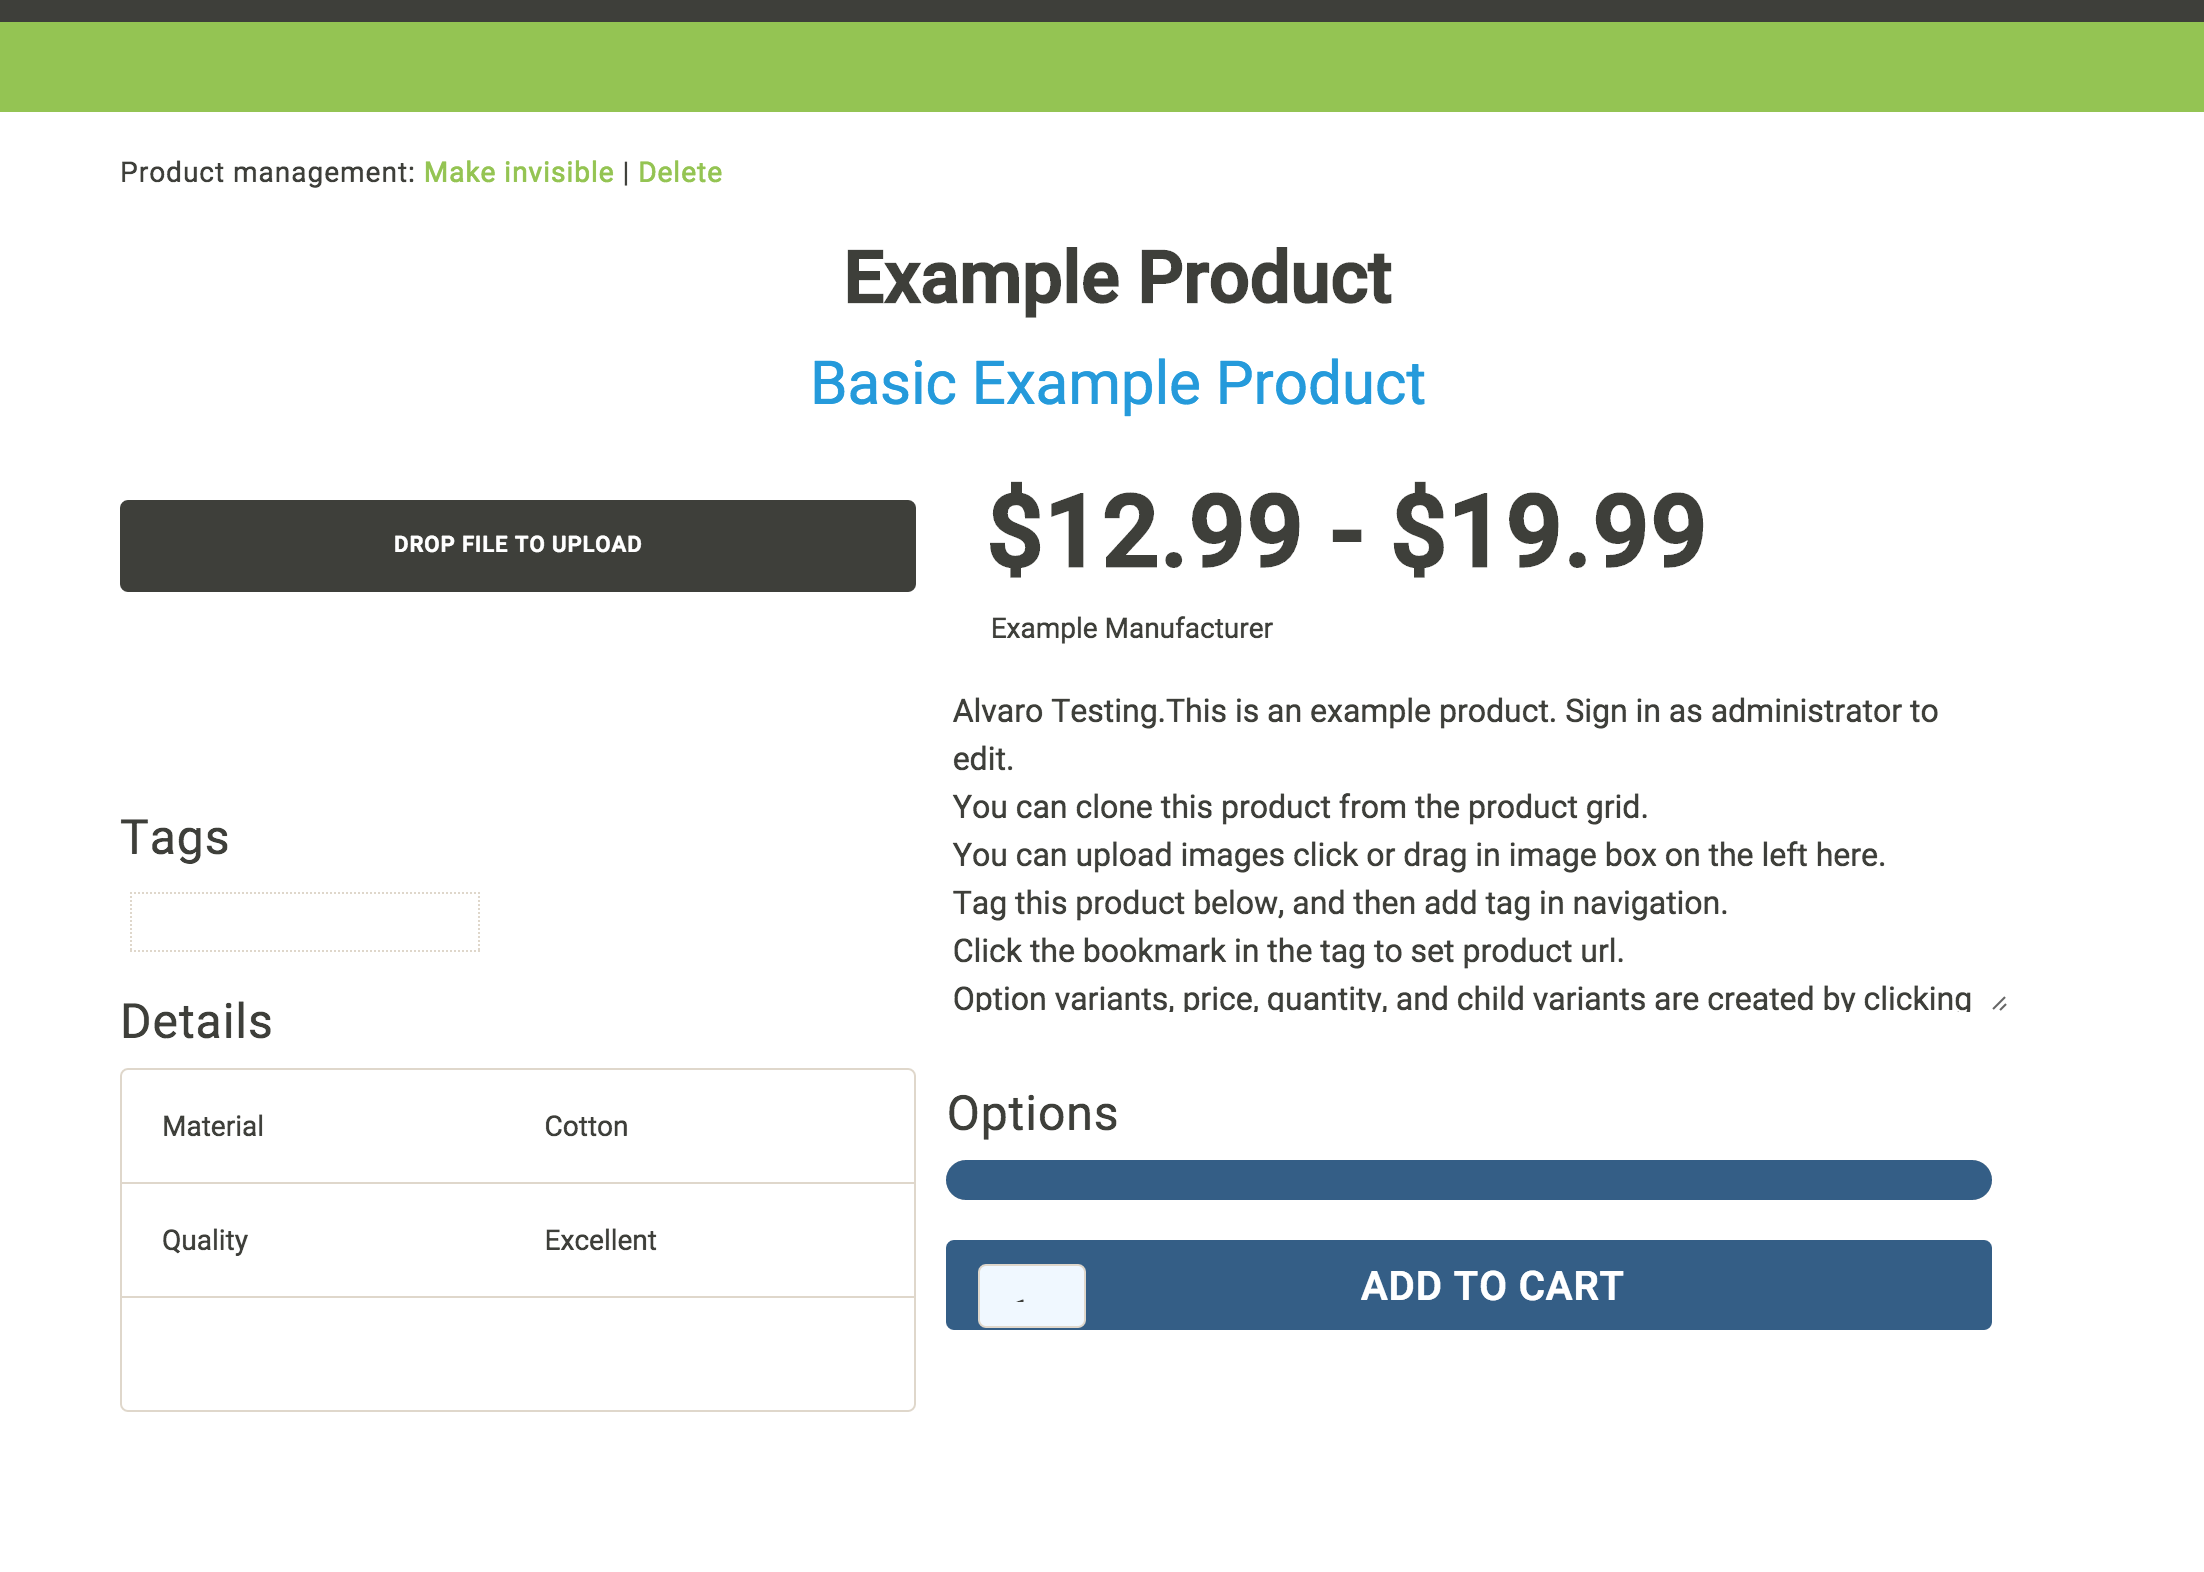
\includegraphics[width=0.8\textwidth]{figuras/productos/interfaz_edicion_producto.png}

% 	\caption{Interfaz de la edición de un producto.}
% 	\label{figure:features:interfaz_edicion_producto}
% \end{figure}

% \begin{figure}[H]
% 	\centering
% 	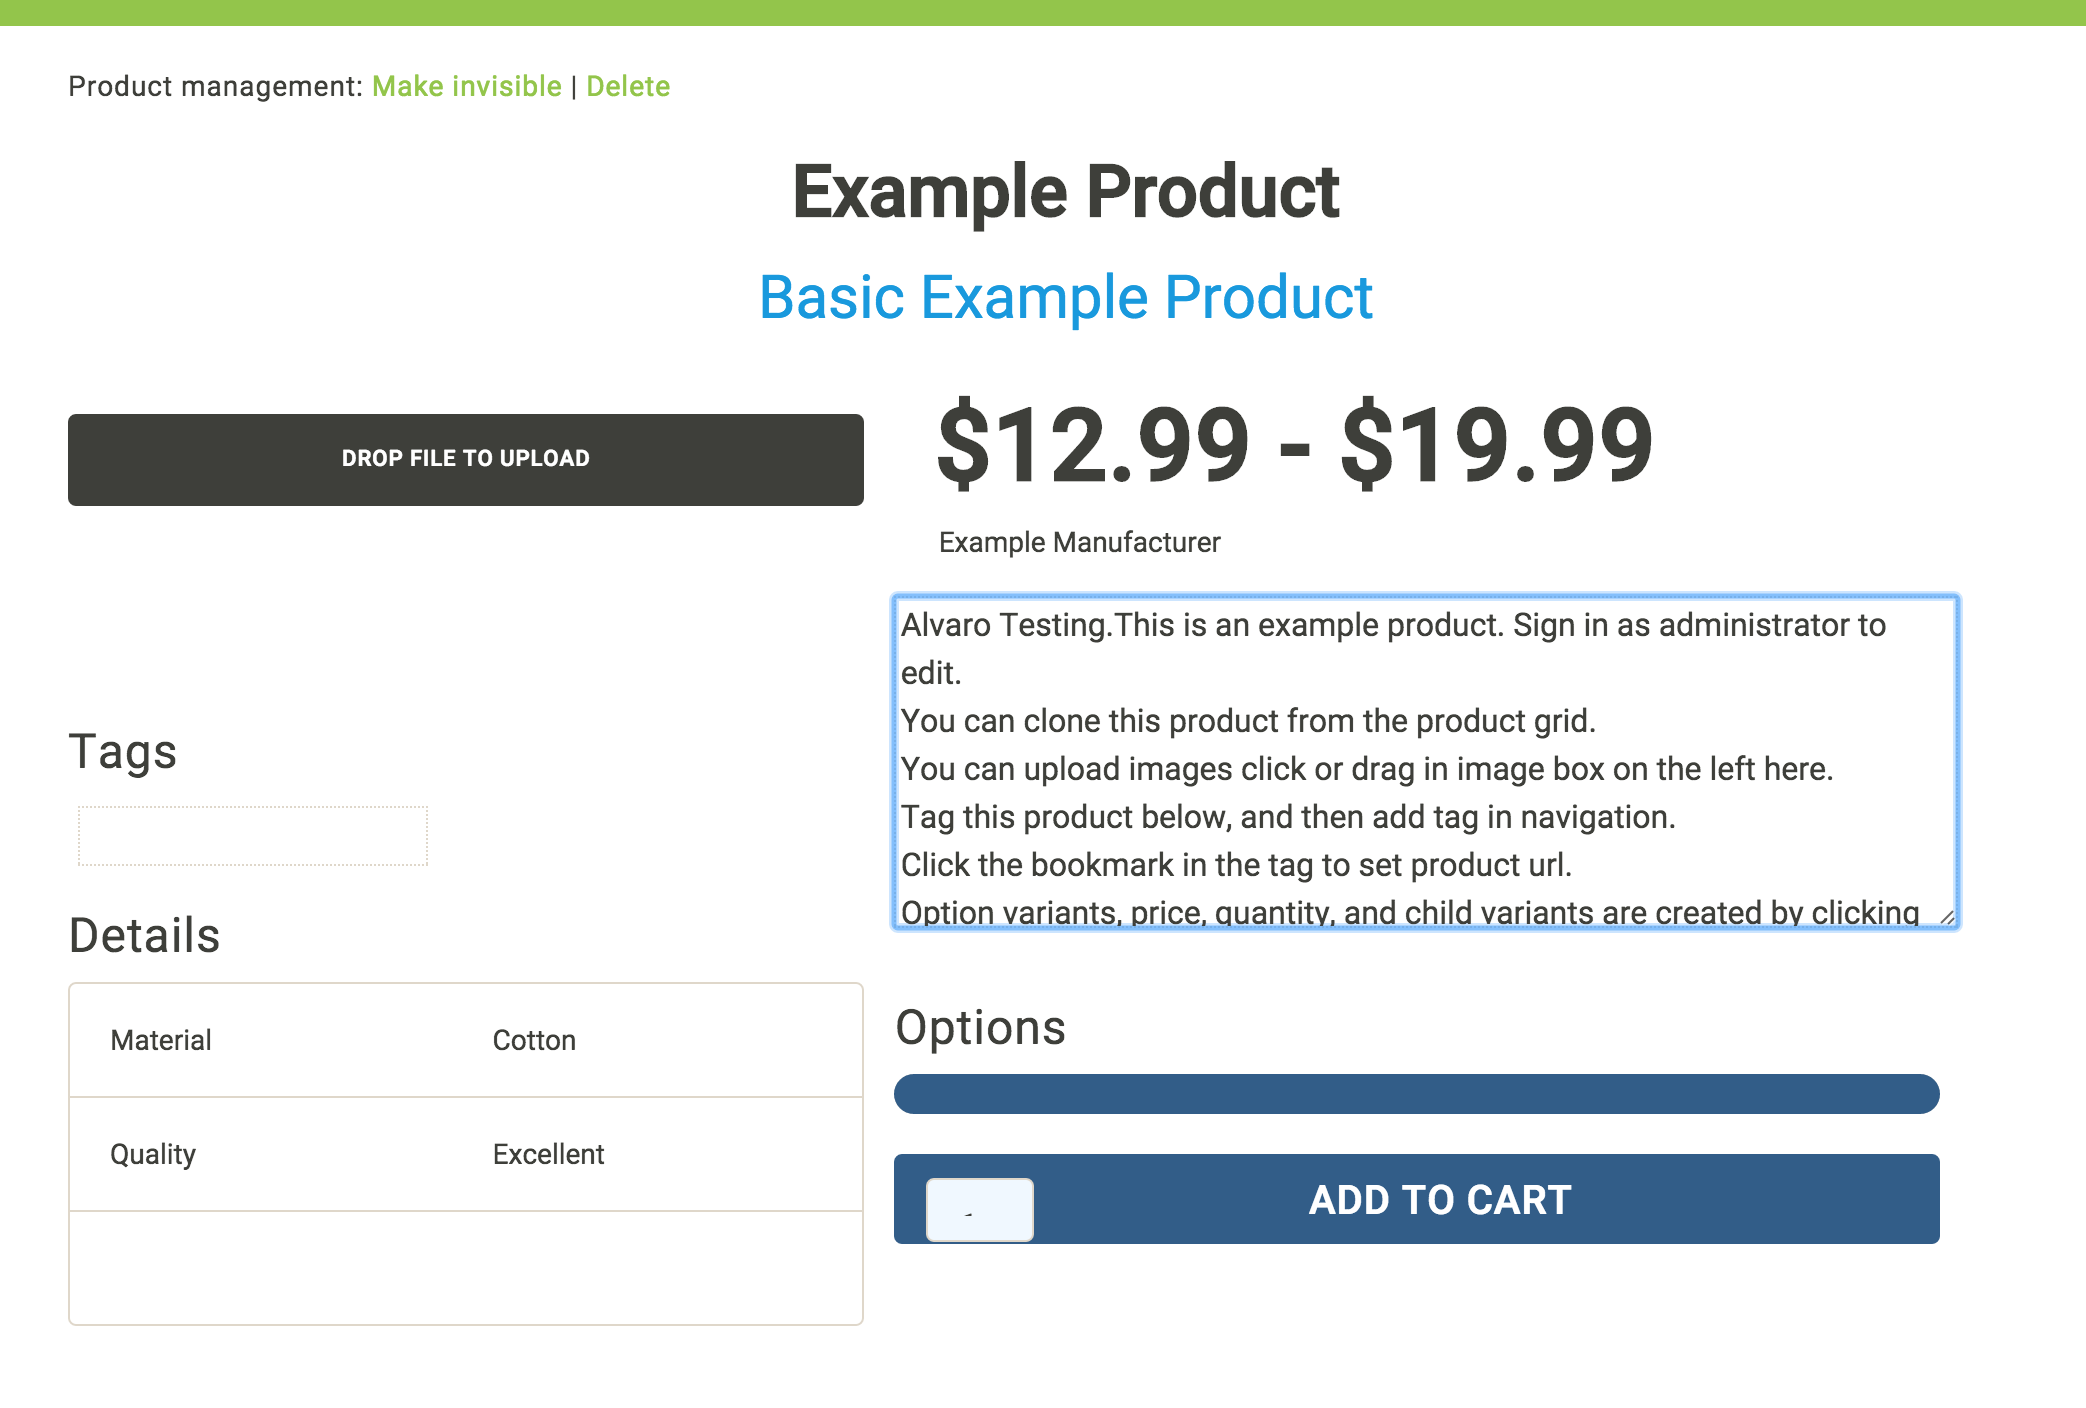
\includegraphics[width=0.8\textwidth]{figuras/productos/interfaz_edicion_editando_description.png}

% 	\caption{Campo descripción seleccionado para edición.}
% 	\label{figure:features:interfaz_edicion_editando_description}
% \end{figure}


% \begin{figure}[H]
% 	\centering
% 	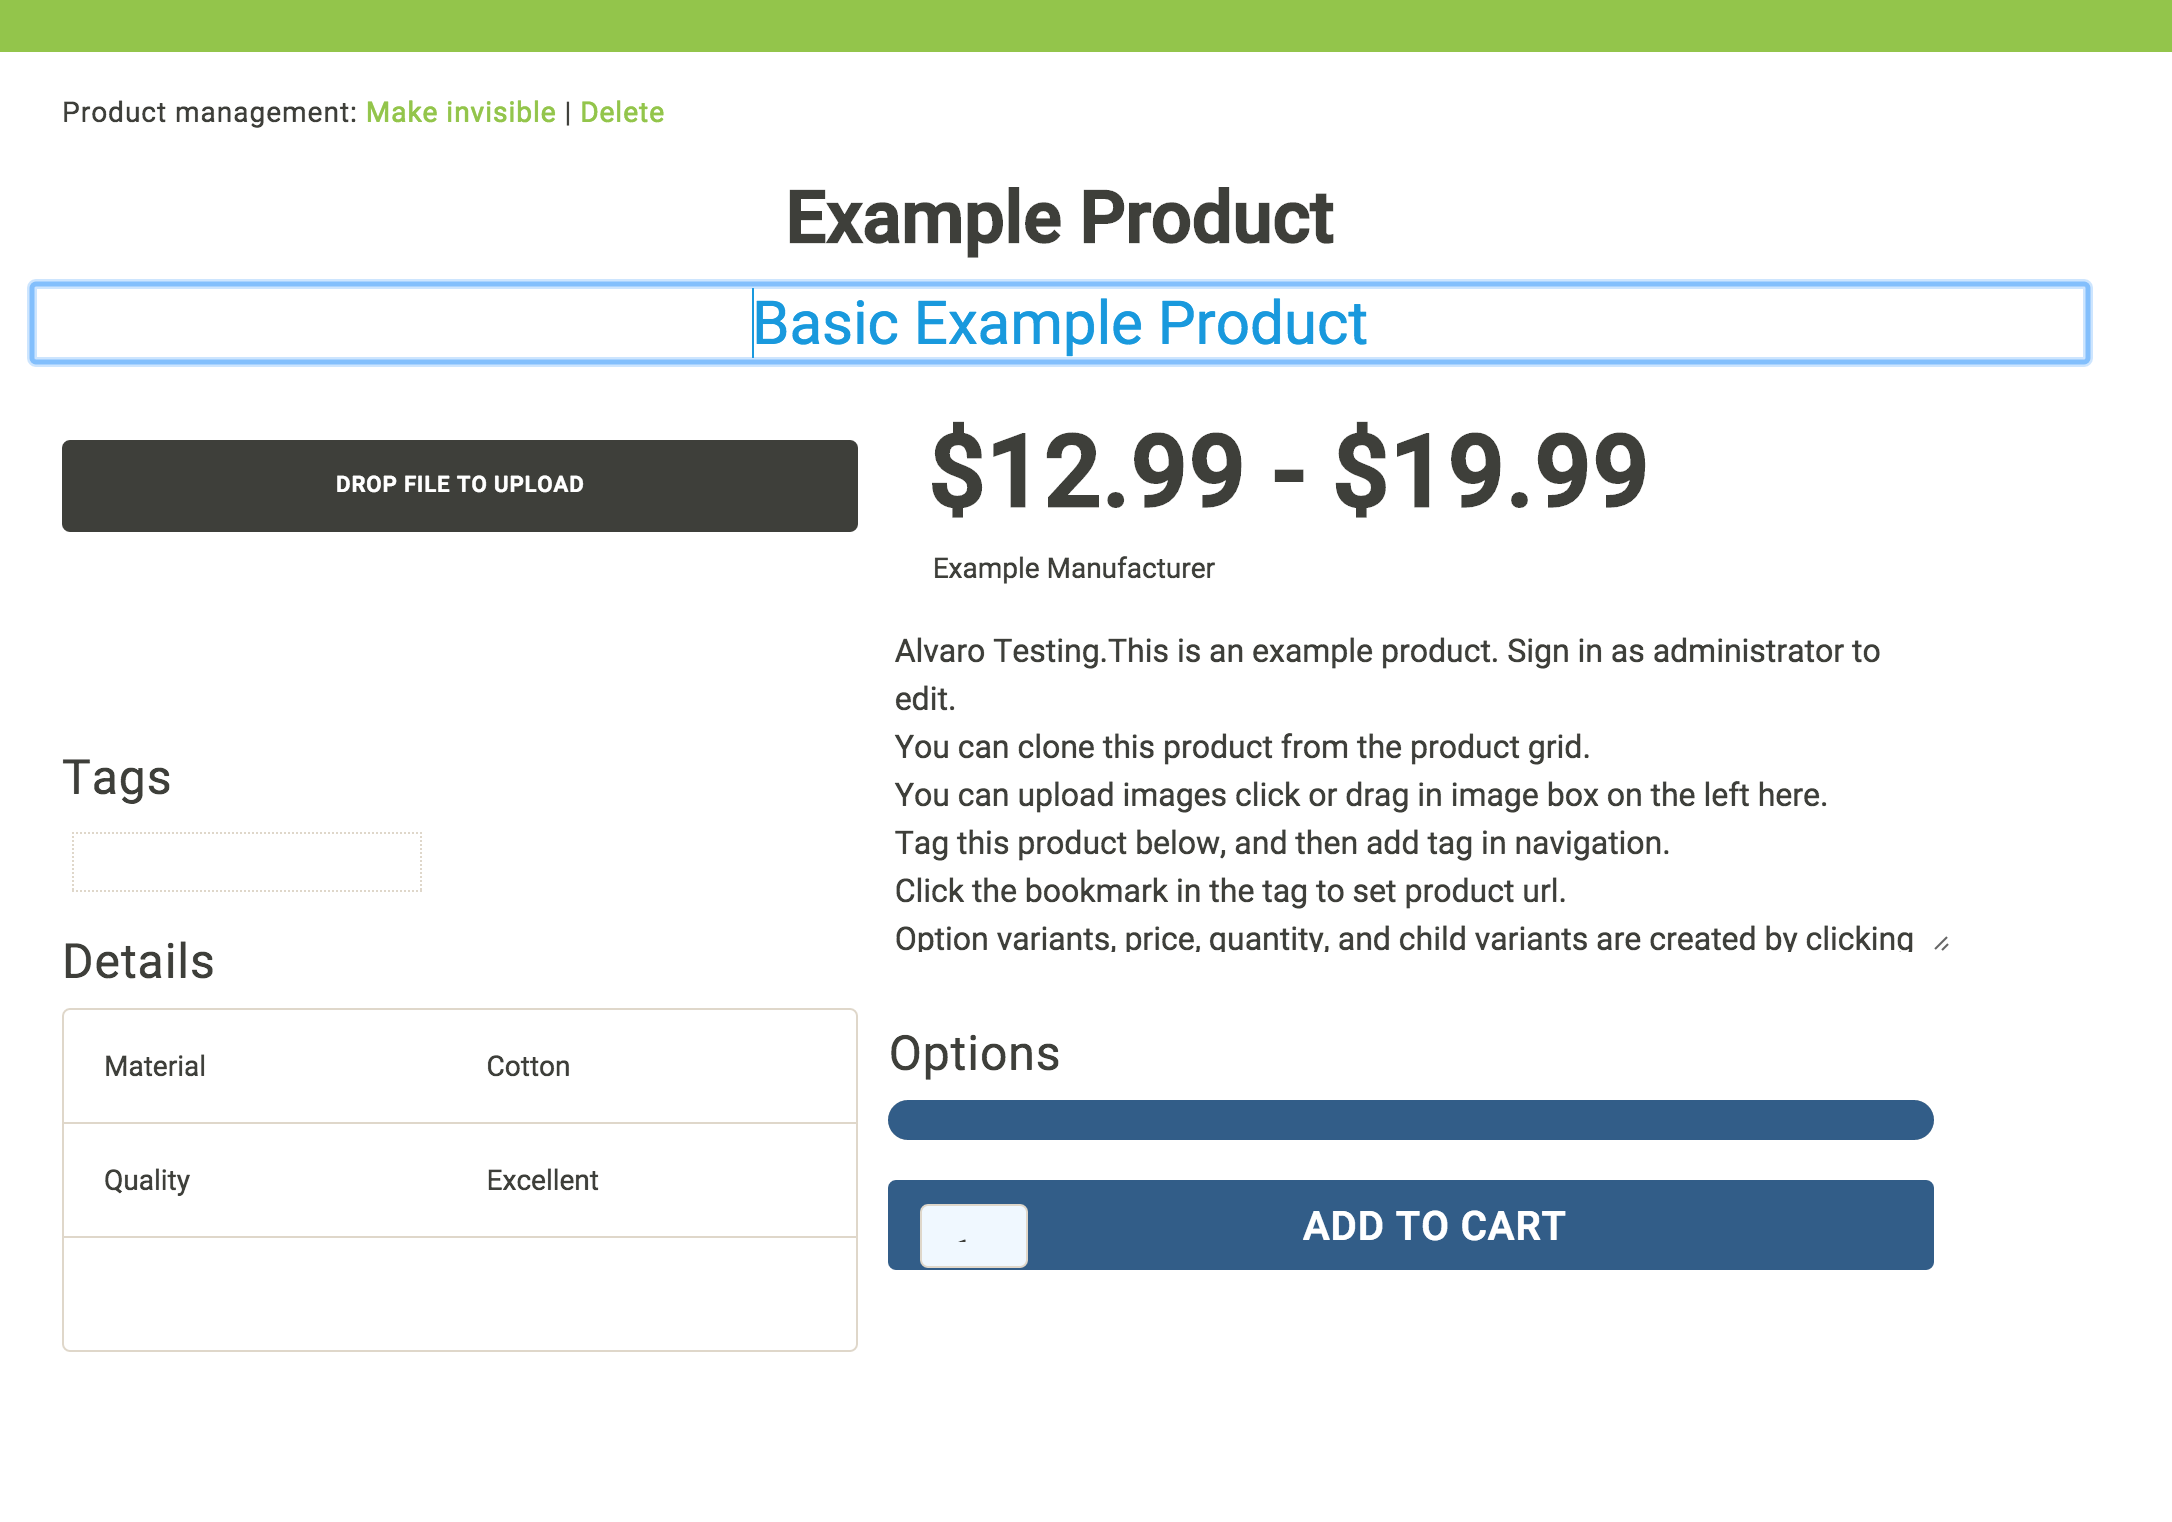
\includegraphics[width=0.8\textwidth]{figuras/productos/interfaz_edicion_editando_subtitulo.png}

% 	\caption{Campo subtítulo seleccionado para edición.}
% 	\label{figure:features:interfaz_edicion_editando_subtitulo}
% \end{figure}

% Es importante mencionar que la edición de producto es \reactive, por lo tanto todos los cambios que se realizen , serán inmediatamente visibles por parte de todos los usuarios que esten mirando la descripción del producto incluso sin la necesidad de que el usuario haga un \refreshCPT del \websiteINT.

% \subsection{\themesCPT}

% Como se explicó en la subsección \ref{chapter:section:subsection:package_core_theme}, la aplicación permite cambiar el \themeCPT utilizando el \packageAS correspondiente.
% Una de las partes más importantes del \frameworkPC \ecommerceCOM corresponde justamente a la customización de la aplicación, dado que esto lograr generar identidad.
% Posteriormente el sistema permitirá además agregar \templatesAS que permita una personalizaciónn del \websiteINT aun más detallada.


\section{\dataModelAS}

Existen \dataModelsAS que se encuentran en una fase avanzada de desarrollo. Recordar que la \dataBaseDB (\mongodbNAME), no tiene \schemasDB estáticos. Esto ha sido particularmente valioso en el proceso de desarrollo de la solución, dado que variados cambios han surgido en el proceso. Estos \dataModelsAS pueden ser revisados en \refApendice{ap:avance_data_model}.

